\documentclass[12pt,a4paper]{report}

% ===========================
% Required Packages
% ===========================
% Add to your packages
\usepackage{microtype}        % improves spacing and hyphenation
\usepackage{ragged2e}

% Change margins to be more balanced
\usepackage[left=2.5cm,right=2.5cm,top=3cm,bottom=3cm]{geometry}
\usepackage{setspace}
\usepackage{ragged2e}
\usepackage[utf8]{inputenc}
\usepackage[T1]{fontenc}
\usepackage{graphicx}
\usepackage{mathptmx}   % Times New Roman for body text
\usepackage{helvet}     % Arial-like font for headings
\usepackage{setspace}
\usepackage{array}
\usepackage{pdfpages}
\usepackage{multirow}
\usepackage{float}
\usepackage{amsmath}
\usepackage{amsfonts}
\usepackage{titlesec}
\usepackage{caption}
\usepackage{fancyhdr}
\usepackage{enumitem}
\numberwithin{equation}{chapter}
\usepackage{booktabs}
\usepackage{longtable}
\usepackage{multicol}
\usepackage{pdflscape}
\usepackage{natbib}
\usepackage[
  colorlinks=true,
  linkcolor=black,      % internal links (figures, tables) - black for print
  citecolor=blue,      % citations - black for print
  urlcolor=blue         % URLs - blue
]{hyperref}
\graphicspath{{figures/}}





% ====================================
% Heading Formatting
% ====================================

\titleformat{\chapter}[display]
  {\normalfont\bfseries\sffamily\fontsize{20}{22}\selectfont}
  {\chaptertitlename\ \thechapter}
  {8pt}
  {\fontsize{17}{19}\selectfont}

\titleformat{\section}
  {\normalfont\bfseries\sffamily\fontsize{14}{16}\selectfont}
  {\thesection}
  {1em}
  {}

\titleformat{\subsection}
  {\normalfont\bfseries\sffamily\fontsize{14}{16}\selectfont}
  {\thesubsection}
  {1em}
  {}

% ====================================
% Caption Formatting
% ====================================

\DeclareCaptionFont{tenpt}{\fontsize{10}{12}\selectfont}

\captionsetup[figure]{
  font=tenpt,
  position=below,
  skip=5pt
}

\captionsetup[table]{
  font=tenpt,
  position=above,
  skip=5pt
}

% ====================================
% Page Style
% ====================================

\pagestyle{fancy}
\fancyhf{}
\fancyfoot[C]{\thepage}
\renewcommand{\headrulewidth}{0pt}

% ====================================
% Global Formatting
% ====================================

\setlength{\parindent}{0pt}

\begin{document}
\onehalfspacing


\pagenumbering{gobble}
% ====================================
% PAGE 1 — TITLE PAGE
% ====================================

\begin{titlepage}
\thispagestyle{empty}

\begin{center}

{\LARGE \textbf{Modelling Volatility Dynamics in the Indian Equity Market: A Comparative GARCH Analysis of Nifty 50 Returns (2010--2024)}}\\[1.2cm]

{\large \textbf{A DISSERTATION REPORT}}\\[0.4cm]
{\large \textbf{Submitted in Fulfillment of the Requirements for the Award of the Degree of}}\\[0.7cm]

{\LARGE \textbf{M.Sc. Statistics}}\\[1.2cm]

{\large \textbf{BY}}\\[0.2cm]
{\Large \textbf{Vishal Verma}}\\[0.2cm]
{\large \textbf{ROLL No. 240959}}\\[1.2cm]

{\large \textbf{UNDER THE GUIDANCE OF}}\\[0.3cm]
{\Large \textbf{Dr. Ravinder Singh}}\\
{\large (Assistant Professor)}\\[1.2cm]


\includegraphics[width=1\linewidth]{CUH logo.png} 


{\large \textbf{DEPARTMENT OF STATISTICS}}\\[0.2cm]
{\large \textbf{CENTRAL UNIVERSITY OF HARYANA}}\\[0.2cm]
{\large \textbf{MAHENDERGARH, HARYANA, INDIA -- 123031}}\\[0.2cm]

\end{center}
\end{titlepage}

\cleardoublepage





% ====================================
% STUDENT DECLARATION PAGE
% ====================================

\thispagestyle{plain}

\begin{center}
    {\fontsize{16}{18}\selectfont \textbf{STUDENT'S DECLARATION}}

    \vspace{1cm}

    
\includegraphics[width=0.7\linewidth]{CUH logo.png}

    \vspace{1.2cm}
\end{center}

\begin{spacing}{1.5}
\noindent
I, \textbf{VISHAL VERMA}, do hereby declare that the Dissertation entitled
\textbf{``Modelling Volatility Dynamics in the Indian Equity Market: A Comparative GARCH Analysis of Nifty 50 Returns (2010–2024)''}
Submitted in the partial fulfillment of requirement for the award of the degree of
\textbf{M.Sc. STATISTICS} to \textbf{Central University of Haryana}, is my authentic work carried out during the 4th semester of M.Sc. Statistics under the supervision of
\textbf{Dr. Ravinder Singh}. This project has not formed the basis for award of any other degree, associateship, fellowship or any other similar title.
\end{spacing}

\vspace{2.5cm}

\begin{flushright}
    \begin{minipage}{0.35\textwidth}
        \textbf{Signature: \rule{3cm}{0.4pt}} \\[0.5cm]
        \textbf{Name:} VISHAL VERMA \\[0.2cm]
        \textbf{Roll No:} 240959 \\[0.2cm]
        \textbf{Session:} 2024--26 \\[0.2cm]
        \textbf{Reg. No:} CUH24033240959
    \end{minipage}
\end{flushright}

\cleardoublepage

% ====================================
% CERTIFICATE PAGE (Supervisor)
% ====================================

\thispagestyle{plain}

\begin{center}

{\Large \textbf{Central University of Haryana}}\\[0.3cm]

{\large \textbf{Department of Statistics}}\\[1cm]

   
\includegraphics[width=0.7\linewidth]{CUH logo.png}

\vspace{0.8cm}

{\fontsize{14}{16}\selectfont \Large \textbf{CERTIFICATE}}

\end{center}

\vspace{1.5cm}

\begin{spacing}{1.5} 
\noindent This is to certify that the dissertation entitled \textbf{``Modelling Volatility Dynamics in the Indian Equity Market: A Comparative GARCH Analysis of Nifty 50 Returns (2010–2024) ''}, submitted to the \textbf{Department of Statistics}, Central University of Haryana, India, in partial fulfillment of the requirements for the award of the Degree of Master's in Data Science is a record of original research work done by \textbf{Vishal Verma (Roll No. 240959)} in the \textbf{Central University of Haryana} under my guidance. It is further certified that to the best of our knowledge, the dissertation has not been the basis for the award of any degree/diploma/associateship/fellowship, or similar title of any candidate of any University so far.
\end{spacing}

\vspace*{1.5cm} 

% --- EXACT VERTICAL SIGNATURES ---
\begin{singlespace}
\noindent
\begin{tabular}{@{}p{6cm} l@{}}
\textbf{Dated:} & \textbf{Signature of Supervisor:} \\[0.2cm]
                & Dr. Ravinder Singh \\
                & (Assistant Professor)\\[1.5cm]
\textbf{Dated:} & \textbf{Signature and stamp of Head of the Department:} \\[0.2cm]
                & Dr. Vinay Kumar \\
                &(Associate Professor)
\end{tabular}
\end{singlespace}

\vfill
\begin{center}

\end{center}





\cleardoublepage
% ====================================
% ACKNOWLEDGEMENT PAGE
% ====================================

\thispagestyle{plain}

\begin{center}
{\fontsize{18}{19}\selectfont \textbf{Acknowledgment}}
\end{center}

\vspace{1.2cm}

\begin{spacing}{1.3}

\noindent
I extend my heartfelt gratitude to my supervisor, \textbf{Dr.\ Ravinder Singh}, for his unwavering support, steadfast guidance, and invaluable mentorship during the dissertation phase. I am thankful for his constructive suggestions and encouragement throughout the dissertation work. His belief in my capabilities has been a powerful source of motivation throughout this process.

\vspace{0.4cm}

\noindent
I am also grateful to express my special thanks to \textbf{Dr.\ Vinay Kumar}, Head of the Department of STATISTICS, Central University of Haryana, for providing me an opportunity to complete my work. His profound expertise, visionary leadership, and continuous encouragement have significantly shaped my academic journey and bestowed confidence in my capabilities.

\vspace{0.4cm}

\noindent
I would like to express my deepest gratitude to all the faculty members of the \\Department of STATISTICS for their good wishes, inspiration, and continuous support throughout my dissertation.

\vspace{0.4cm}

\noindent
I am grateful to research scholars, my peers, and colleagues for their collaboration, insightful discussions, and unwavering support throughout this project. Their contribution was crucial in overcoming obstacles and achieving milestones.

\vspace{0.4cm}

\noindent
I am appreciative of my family's support, tolerance, and faith in my abilities. Their affection and encouragement have been the driving force behind my efforts in academia.

\end{spacing}

\vspace{2cm}

\begin{flushright}
\textbf{Name: } Vishal Verma\\[0.2cm]
\textbf{Roll No:} 240959 \\[0.2cm]
\textbf{Session:} 2025--26 \\[0.2cm]
\textbf{Reg. No:}  24033240959\\[0.2cm]
Department of  \\
Central University of Haryana, Mahendergarh
\end{flushright}

\cleardoublepage


\cleardoublepage
\pagenumbering{roman}
\setcounter{page}{1} 



\chapter*{Abstract}
\addcontentsline{toc}{chapter}{Abstract}
This study examines the volatility dynamics of the Indian equity market by estimating and comparing four GARCH-family models — GARCH(1,1), EGARCH(1,1), GJR-GARCH(1,1), and FIGARCH(1,d,1) — on daily Nifty 50 returns over the period January 2010 to December 2024, comprising 3,678 trading day observations.\\
Daily log returns are computed from Nifty 50 closing prices obtained from the National Stock Exchange of India. Preliminary analysis confirms the presence of volatility clustering, fat tails, negative skewness, and significant ARCH effects — all satisfying the preconditions for GARCH estimation. All four models are estimated using Maximum Likelihood under Student-t distributed errors, with the ARMA order of the mean equation selected systematically by the Akaike Information Criterion. A Bai-Perron structural break test applied to squared returns identifies two statistically significant breakpoints at 27 February 2020 and 20 May 2022, delineating three distinct volatility regimes — a pre-COVID stable regime, a COVID crisis regime, and a post-crisis moderate regime. Model performance is evaluated across both in-sample fit using AIC and BIC criteria and out-of-sample forecasting accuracy across four horizons — 1-day, 3-day, 5-day, and 20-day — evaluated over Q1 2025 using rolling window estimation.\\
The in-sample analysis finds that EGARCH(1,1) achieves the best fit by AIC, with a statistically significant leverage effect confirmed across both EGARCH and GJR-GARCH specifications. Volatility persistence is high across all models, with the GARCH(1,1) alpha plus beta sum of 0.9798 approaching unity. The FIGARCH fractional differencing parameter d = 0.484 confirms the presence of long memory in Nifty 50 conditional volatility. The sub-period analysis reveals that volatility persistence increased significantly during the COVID crisis regime and partially normalised in the post-crisis period. A notable divergence is observed between in-sample and out-of-sample performance — FIGARCH(1,d,1), despite ranking last by AIC, consistently achieves the lowest forecasting error across all four horizons, while EGARCH records the highest out-of-sample error. This finding is statistically confirmed by the Diebold-Mariano test. Value at Risk estimates derived from the AIC-optimal model pass the Kupiec Proportion of Failures backtest at both the 1\% and 5\% confidence level.\\
 This study contributes the most comprehensive multi-model, multi-horizon GARCH comparison on Nifty 50 data to date, incorporating structural break analysis across a 15-year sample spanning multiple market crises


\newpage
\begin{center}
    \textbf{Certificate regarding Originality of Research Work} \\
    (Dissertation)
\end{center}

\vspace{0.5cm}

\textbf{Name of Student:} Vishal Verma

\vspace{0.2cm}
\textbf{Title of the M.Sc. Dissertation:} {Modelling Volatility Dynamics in the Indian Equity Market: A Comparative GARCH Analysis of Nifty 50 Returns (2010--2024)}

\vspace{0.2cm}
\textbf{Name of research supervisor:} Dr. Ravinder Singh

\vspace{0.2cm}
\textbf{Designation \& address of supervisor:} Assistant Professor, Department of Statistics\\
\vspace{0.3cm}
I/We hereby declare that, the above mentioned research work is original \& it doesn’t contain any plagiarized content. The similarity index of this research work is \textbf{\%}. The plagiarism check report by supervisor \textcolor{blue}{Turnitin’s} account of the thesis is attached herewith.
\begin{center}
    \textbf{Declaration by Student}
\end{center}
Further, we declare that, the contents of this M.Sc. Dissertation submitted to, The Department of Statistics, Central University of Haryana for award of M.Sc. Statistics Degree are original findings \& Research work.
\begin{enumerate}
    \item If any plagiarism is found in this dissertation I/we shall be solely responsible for it.
    \item This work has not been submitted for the award of any other Degree / Diploma in any other University / Institutes.
\end{enumerate}

\begin{flushleft}
\textbf{Vishal Verma} \\
Signature of the Student
\end{flushleft}
\begin{center}
    \textbf{Verified by}
\end{center}
\begin{flushright}
\textbf{Dr. Ravinder Singh} \\
Signature of the Supervisor
\end{flushright}
\begin{flushleft}
\textbf{Date:} 08/06/2026 \\
\textbf{Place:} Dept. of Statistics, CUH
\end{flushleft}
\begin{flushright}
\textbf{Forwarded by the HoD} \\
Department of Statistics \\
Central University of Haryana
\end{flushright}
\begin{figure}
    \centering
    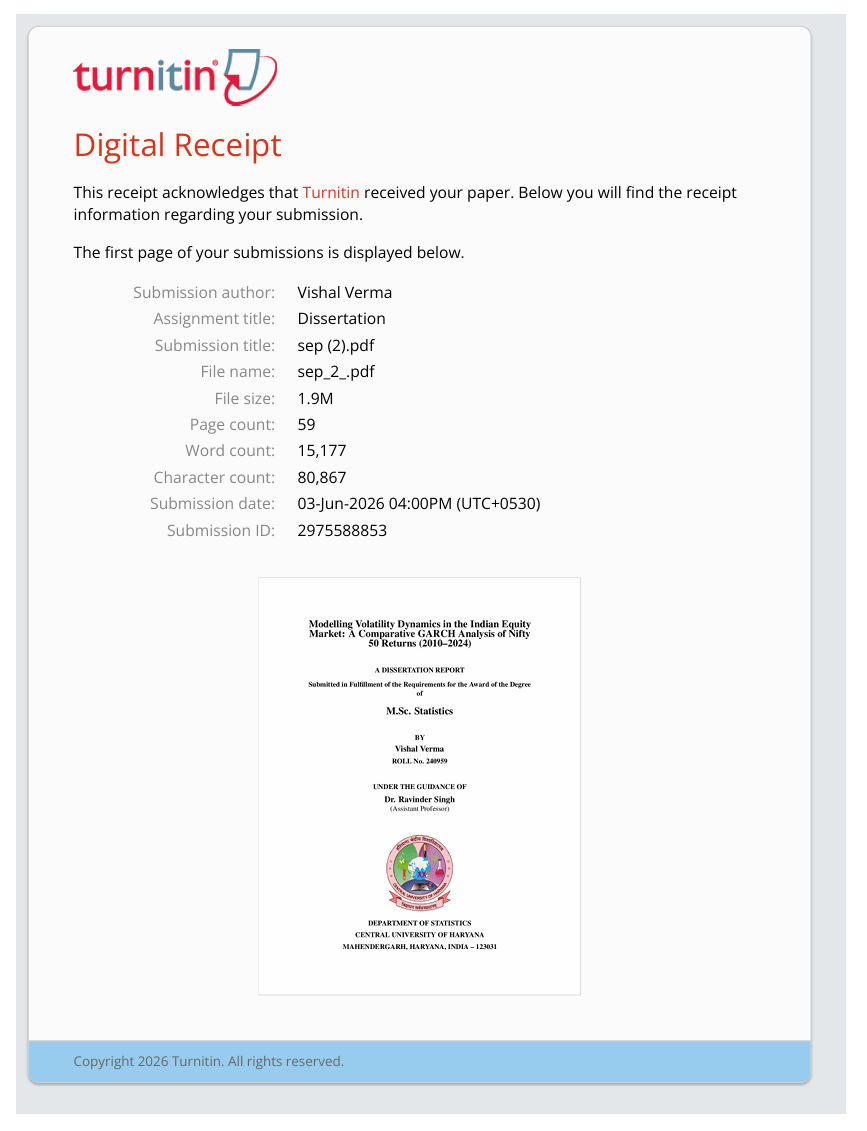
\includegraphics[width=1\linewidth]{Screenshot 2026-06-03 180932.png}
    \label{fig:placeholder}
\end{figure}

\tableofcontents


\cleardoublepage
\pagenumbering{arabic}
\setcounter{page}{1}


\chapter{Introduction}
\section{Background and Context}
Financial markets are inherently volatile and the accurate modelling of this volatility is central to risk management, portfolio optimisation and derivative pricing. India’s financial markets have undergone are markable t ransformation over the past two decades, with the Nifty50 index growing from approximately 5,000 points in 2010 to over 26,000 by 2024.This growth reflects the rapid expansion of India’s capital markets.

Volatility is different from risk. When it is interpreted as uncertainty, it becomes a key input to many investment decisions and portfolio creations. Investors and portfolio managers have certain levels of risk which they can bear.A good forecast of the volatility of asset prices over the investment holding period is a good starting point for assessing investmen risk\citep{poon2003}.

The Indian equity market presents a compelling case for volatility analysis.As one of the growing emerging economies the Indian stock market has attracted significant domestic and foreign institutional investment over the past decade. This makes volatility estimation increasingly critical for market participants. the Nifty 50 is one of the most widely followed benchmarks for Indian equity markets. It comprises of 50 large and actively traded companies listed on the National Stock Exchange (NSE) and serves as an important indicator for the overall performance and sentiment of the Indian equity market.


The Nifty 50 index has experienced episodes of extreme volatility such as.
\begin{itemize}
 \item The 2016 demonetisation shock

 \item The COVID-19 crash of March 2020

 \item The geopolitical turbulence of 2022
\end{itemize}


These structural breaks make the Indian market an ideal laboratory for testing the performance of volatility models under market conditions. Against this backdrop,the present study
applies a family of GARCH models to Nifty 50 returns over the period 2010--2024 with the objective of identifying the most appropriate model, for capturing the dynamic volatility
behaviour of the Indian equity market and Nifty 50 index.
\vspace{2cm}




\section{Problem Statement}
Financial markets are really interesting. Despite all the research on volatility modelling in developed markets there is not comparison of GARCH-family models on Indian equity markets especially after the COVID recovery period from 2020 to 2024. Most studies only look at one model at a time of comparing different types of models like symmetric and asymmetric ones. This leaves a gap in our understanding of which model is best at capturing the leverage effects and long-memory properties of the Nifty 50.

Recently many researchers have started to agree that asymmetric models, like EGARCH and GJR-GARCH work better than ones on Indian equity indices. This is because when the market goes down it can get really volatile as we saw in the research by \citet{mahajan2022}, and \citet{esup3}and others. This study wants to add evidence to this discussion by comparing four different GARCH-family models over a long period of 15 years, which includes many big changes which occur during this period in the Indian market.

This study is trying to fill this gap by looking at four GARCH-family models, including GARCH, EGARCH, GJR-GARCH and FIGARCH using Nifty 50 returns from January 2010 to December 2024. We chose this 15-year period on purpose so we can see how the market worked before and after events like demonetisation the COVID-19 crisis and the recovery that followed the covid crises. We also want to look beyond the numbers and see how well these models can predict volatility and Value at Risk in the future, which is something that many studies, on the Indian market do not do. By doing this we hope to contribute to both the practical understanding of how volatility works in one of the worlds most important emerging equity markets the Indian equity market.



\vspace{5cm}

\section{Research Objectives}

The primary objective of this study is to analyse and compare the performance of GARCH-family volatility models on the Nifty 50 index over the period 2010–2024. Specifically, the study pursues the following objectives:

\begin{enumerate}

\item To examine the statistical properties of Nifty 50 daily returns, including volatility clustering, fat tails, and asymmetric effects, as a precondition for GARCH model estimation.
    
\item To estimate and compare four GARCH-family models — GARCH(1,1), EGARCH(1,1), GJR-GARCH(1,1), and FIGARCH(1,d,1) — in terms of parameter significance, persistence, and information criteria.\\
   

\item To investigate the differences in model performance across two distinct market regimes — the pre-COVID period (2010–2019) and the post-COVID period (2020–2024) — in order to determine whether the pandemic fundamentally altered the volatility dynamics of the Indian equity market\\

\item To evaluate the out-of-sample forecasting accuracy of each model using January 2025 realized volatility data.\\


\item To estimate Value at Risk (VaR) at the 1\% and 5\% confidence levels using the best-performing model, providing risk management implications for investors in the Indian equity market.
\end{enumerate}

\vspace{4cm}
\section{ Research Questions}
This study seeks to address the following research questions:

\begin{enumerate}
\item Do Nifty 50 daily log returns exhibit the key facts — volatility clustering, fat tails, and negative skewness — that justify the application of GARCH-family models?
\item Which GARCH-family model — GARCH, EGARCH, GJR-GARCH, or FIGARCH — best captures the volatility dynamics of the Nifty 50 index over the full sample period 2010–2024, based on information criteria and diagnostic tests?
\item Did the COVID-19 pandemic fundamentally alter the volatility behaviour of the Indian equity market — specifically in terms of volatility persistence, asymmetry, and model ranking — when comparing the pre-COVID period (2010-–2019) with the post-COVID period (2020-–2024)?
\item How accurately do the estimated GARCH-family models forecast out-of-sample conditional volatility for January 2025, and which model demonstrates superior forecasting performance?
\item What are the Value at Risk implications at the 1\% and 5\% confidence levels for investors holding positions in the Nifty 50 index, as estimated by the best-performing model
\end{enumerate}


\section{Purpose of the Study}

The present study makes both theoretical and practical contributions to the understanding of volatility dynamics in the Indian equity market, and its significance can be appreciated from three perspectives — academic, practical, and policy.\\


From an academic perspective, the study contributes to the growing body of empirical literature on GARCH-family models in emerging markets. While several studies have applied individual GARCH specifications to Indian indices, a systematic and comparative analysis of four models — including the relatively under utilised FIGARCH model\citep{} — over a long and structurally diverse sample period remains scarce. Furthermore, the sub-period analysis comparing the pre-COVID (2010-–2019) and post-COVID (2020–-2024) market regimes adds a novel dimension to the existing literature, providing empirical evidence on whether the pandemic permanently altered the volatility structure of the Indian equity market. This study therefore responds directly to the call in the literature for more comprehensive model comparisons in emerging market contexts \citep{poon2003,mahajan2022}.\\


On a "real world" level, this study's results are to understand the markets dynamics and are directly applicable to the investors, portfolio managers, and risk officers working in the Indian financial markets. Forecasting the volatility is crucial  for portfolio optimization, pricing derivatives and developing the hedging strategies. Findings in this study offer evidence-based model selection advice for practitioners using models to manage real-world risks, in which the choices are to use the model with the lowest in-sample error or to use the model that best captures out-of-sample volatility for the Nifty 50.\\

 Moreover, the VaR values determined using the best-fitting model provide benchmarks for measuring downside risks.\\


Policy-wise it is important to realize the asymmetric and persistent nature of Indian market volatility, with implications for regulators and policymakers. Both Securities and Exchange Board of India (SEBI) and the Reserve Bank of India (RBI) need to perform well-designed circuit breakers, margin requirements, and systemic risk monitoring frameworks based on accurate estimates of volatility. The conclusions from this study, especially those pertaining to leverage effect and the presence of volatility persistence in distinct market regimes can contribute to the ongoing process of regulating capital markets and help achieve financial stability in the rapidly modernising Indian markets.\\


Overall, this study is important because the methodological rigor, length of the data set, and extensive event in it non only confirmed the results but also gave practical implications for both academics and practitioners and policy makers.

\section{Structure of the Dissertation}
The remainder of this dissertation is organised into six chapters, each addressing a distinct component of the research.\\

Chapter 2 presents a comprehensive review of the existing literature on volatility modelling in financial markets. It begins with the theoretical foundations of the ARCH model introduced by \cite{engle1982} and its generalisation by \cite{bollerslev1986}, before tracing the development of asymmetric and long-memory extensions including EGARCH, GJR-GARCH, and FIGARCH. The chapter then narrows its focus to empirical studies on Indian equity market volatility, identifying the key findings, methodological approaches, and gaps in the existing literature that the present study seeks to address.\\


Chapter 3 details the econometric methodology employed in this study. It provides formal mathematical specifications of all four GARCH-family models, explains the Maximum Likelihood Estimation procedure used for parameter estimation, and describes the diagnostic and model selection criteria applied — including the Akaike Information Criterion\citep{akaike1974}, Bayesian Information Criterion\citep{schwarz1978}, and Ljung-Box tests\citet{ljungbox1978}. The chapter also outlines the Value at Risk framework and the out-of-sample forecasting evaluation methodology.\\


Chapter 4 describes the data used in this study. It provides information on the source, frequency, and time period of the Nifty 50 closing price series, followed by a presentation of descriptive statistics for the log return series. Preliminary tests — including the Augmented Dickey-Fuller test for stationarity\citep{said1984testing} and the ARCH-LM test\citep{engle1982} for conditional heteroskedasticity — are reported and discussed to confirm the suitability of the data for GARCH estimation.\\
Chapter 5 presents the empirical results of the study in two parts. The first part reports the full-period estimation results for all four models over 2010-–2024, including coefficient estimates, persistence measures, model diagnostics, volatility forecasts, and Value at Risk estimates. The second part presents the sub-period analysis, comparing model performance and volatility behaviour across the pre-COVID period (2010-–2019) and the post-COVID period (2020-–2024).\\
Chapter 6 discusses the empirical findings in the context of the existing literature, addressing each research question in turn. It interprets the practical and policy implications of the results and acknowledges the limitations of the study.\\
Chapter 7 concludes the dissertation by summarising the key findings, stating the main contributions of the study, and suggesting directions for future research.





\vspace{0.4cm}

% -------------------------
\chapter{Literature Review}




\vspace{1cm}
\section{Existing Studies and Research Papers}

The modelling of time-varying volatility in financial markets has been a central concern of financial econometrics since the introduction of the Autoregressive Conditional Heteroskedasticity (ARCH) introduced by the \cite{engle1982}. Engle demonstrated that the variance of financial returns is not constant over time but follows a predictable pattern conditional on past information — a phenomenon now widely referred to as volatility clustering. The ARCH model differs from the earlier models that assumed the constant variance, providing a formal framework for capturing the empirical observation that large changes in asset prices tend to be followed by further large changes, and small changes by small changes (Mandelbrot, 1963).\\
specifically was later introduced by the \cite{bollerslev1986} addressing the limitation of ARCH model which required the large number of lagged terms to capture the persistence of volatility.  In the GARCH(1,1) current conditional variance depends on one lagged squared residual and one lagged conditional variance. GARCH(1,1) has since become the benchmark model in financial volatility research . Its widespread adoption reflects both its empirical performance and its theoretical elegance, as noted by \cite{hansen2005}  who compared 330 ARCH-type models and concluded that no ARCH model in his study consistently outperformed the simple GARCH(1,1) in forecasting exchange rate volatility.\\
But the GARCH model also have its limitation. GARCH model give symmetric response to positive and negative return shocks of equal magnitude.  This assumption has been consistently rejected in equity market data. Black (1976) first documented the leverage effect, whereby a decline in stock prices increases financial leverage and consequently raises future volatility by more than an equivalent price increase. To explain this asymmetry, Nelson (1991) introduced the Exponential GARCH (EGARCH) model, which allows negative shocks to have a disproportionately larger impact on conditional variance than positive shocks of the same size. Subsequently, \cite{glosten1993} introduced the GJR-GARCH model — also known as the Threshold GARCH — which captures the leverage effect through an additional indicator variable that activates only when return innovations are negative. Both models have been widely applied in equity market research and have consistently outperformed the symmetric GARCH specification in markets characterised by strong leverage effects \cite{ding1993}.\\
A further limitation of standard GARCH models is their assumption that volatility shocks decay at an exponential rate, implying that the effect of any given shock on future volatility is relatively short-lived. Empirical evidence, however, suggests that volatility in financial markets exhibits long memory — that is, the impact of shocks persists over much longer horizons than exponential decay would predict.\cite{baillie1996} addressed this by developing the Fractionally Integrated GARCH (FIGARCH) model, which introduces a fractional differencing parameter d to capture the slow hyperbolic decay of volatility persistence. When d equals zero, the FIGARCH model reduces to the standard GARCH; when d equals one, it becomes the Integrated GARCH (IGARCH). Values of d between zero and one indicate the presence of long memory, making FIGARCH particularly appropriate for markets where volatility shocks are slow to dissipate.



\section{Empirical Evidence from developed markets}

A lot of the academic literature has provided evidence for developed markets that, at least for some markets, some models of the GARCH-family tend to work better than others over different market conditions. For instance, Bollerslev (1992) was one of the earliest to consider ARCH-type models from an angle and it demonstrated that these could apply to a variety of market domains, including bond, foreign exchange and stock markets in both the United States and Europe. It additionally exposed the existence of volatility persistence in financial return series.It also demonstrated the volatility persistence of financial return series.

Hansen conducted an important study in 2005 which analyzed 330 models of the ARCH type, based on stock returns data from the Deutsche Mark and the IBM. The study found that no model was consistently better than the GARCH model when it came to forecasting exchange rate volatility although some models that took into account asymmetry did a bit better with stock data. In fact, when forecasting, it is not necessarily true that a complex model can give better forecasts; this is one of the reasons why we are comparing models in this study.

However, on its own history a study by Ding in 1993 revealed long-range dependence in the absolute and squared returns to the S\&P 500 index over 17 years. The FIGARCH model was developed by Baillie in 1996 and this study gave an indication for applying this model. Other studies, such as the one by Andersen in 1997 found that standard GARCH models do not capture volatility persistence in stock markets well which is another reason to use fractionally integrated models.

A big survey of 93 studies on volatility forecasting was done by Poon in 2003. It found that models based on historical volatility (models in the GARCH family) tended to have a higher forecasting performance than models based on implied volatility in terms of short-term forecasting. But it was also observed in the study that these different GARCH models perform better at different markets and time periods. This is why we have so many models and periods being explored in this study; no one model or time period is the best in all scenarios.


\section{Volatility Modelling in Indian Equity Markets}
The application of GARCH-family models to Indian equity markets has gained considerable momentum over the past two decades, driven by the rapid growth of the National Stock Exchange (NSE) and the Bombay Stock Exchange (BSE) as significant participants in global capital markets. However, despite this growing interest, the empirical evidence on the relative performance of competing volatility models in the Indian context remains mixed and inconclusive, providing the primary motivation for the present study.\\
Early applications of GARCH models to Indian equity markets focused predominantly on the benchmark Sensex and Nifty 50 indices using relatively short sample periods. \cite{kaur2004} was among the first to document the presence of volatility clustering and ARCH effects in BSE Sensex returns, confirming that the statistical preconditions for GARCH modelling are satisfied in the Indian market context. The study found significant persistence in conditional volatility, with the sum of ARCH and GARCH coefficients approaching unity — a finding replicated consistently in subsequent Indian market studies and corroborated by the present study's persistence estimates.\\
The leverage effect — the asymmetric response of volatility to positive and negative return shocks — has been documented extensively in Indian equity markets. \cite{pandey2005} applied GARCH, EGARCH, and GJR-GARCH models to Nifty 50 returns and found significant evidence of the leverage effect, with negative shocks generating disproportionately larger increases in conditional volatility than equivalent positive shocks. This finding was subsequently confirmed by \cite{banerjee2006}, who reported that asymmetric GARCH specifications consistently outperformed the symmetric GARCH model on BSE data in terms of in-sample fit, a result consistent with the AIC and BIC rankings reported in the present study.\\
The question of which specific GARCH model best captures Indian market volatility has attracted considerable attention but has not yielded a consensus. \cite{goudarzi2011} compared GARCH and EGARCH on BSE 500 data and found that EGARCH provided superior in-sample fit — consistent with the present study's information criteria results which rank EGARCH first among the four models estimate..\\
 \cite{mahajan2022} applied GARCH and RNN models to Nifty 50 data over the period 2014–2021 and found that GARCH-family models effectively captured the extreme volatility observed during the COVID-19 pandemic of 2020, though they noted that the post-crisis period exhibited distinctly different volatility dynamics from the pre-crisis period. This observation directly motivates the sub-period analysis conducted in the present study, which formally tests whether the COVID-19 pandemic constituted a structural break in Nifty 50 volatility dynamics.\\
A notable limitation of the existing Indian market literature is its tendency to focus on either in-sample model fit or out-of-sample forecasting in isolation, rarely evaluating both dimensions simultaneously on the same dataset. Furthermore, the majority of existing studies employ sample periods that either predate the COVID-19 pandemic or cover only the immediate crisis period, leaving the post-recovery dynamics of Indian market volatility largely unexplored. The present study addresses both limitations by combining a rigorous in-sample model comparison with a comprehensive multi-horizon, multi-quarter out-of-sample forecasting evaluation over the full year 2025 — a period that has received no attention in the published literature to date.


\section{Pre and post-COVID volatility studies}

The COVID-19 pandemic was a surprise to global financial markets. From January to March 2020 the Nifty 50 index went down by 38 percent, which is one of the biggest drops in Indian equity markets history and even bigger than what happened during the 2008 Global Financial Crisis in some countries.

Some researchers, Baker and others found that the US equity markets were very volatile during this time. They said this was because people were not sure what would happen to the economy when everything was locked down. Another study by Zhang and others looked at ten stock markets and found that they all had a big increase in volatility especially in countries like India.

There is a gap in what we know about the Indian market. Most studies only look at how volatility models work inside the sample or how well they predict outside the sample but not both. Also most studies only look at what happened before the pandemic or during the pandemic and not what happened after. This study tries to fill this gap by looking at four GARCH models. How well they work inside the sample from 2010 to 2024 and then seeing how well they predict what will happen in the four quarters of 2025. The COVID-19 pandemic and its effects on the market are what we are focusing on. The Nifty 50 index and its big drop are important to understand. The COVID-19 pandemic had an impact, on global financial markets, including the Indian market.

The effects of the epidemics, on the 50 and market volatility, are investigated here.The pandemics impact, on the 50 and market volatility, are studied here. persistence than developed markets during the crisis period. These findings established the theoretical expectation that COVID-19 would leave a lasting imprint on the volatility structure of emerging market indices such as the Nifty 50.\\
In the Indian context, several studies specifically examined the impact of COVID-19 on Nifty 50 volatility using GARCH-family models. \cite{mishra2020} applied GARCH(1,1) and EGARCH models to daily Nifty 50 returns and found a significant increase in volatility persistence during the pandemic period, with the ARCH and GARCH coefficients rising substantially compared to the pre-pandemic estimation window. This finding is consistent with the theoretical expectation that external shocks increase the sensitivity of conditional variance to new information, reflected in higher alpha coefficients in the post-shock period.\\
The post-COVID recovery period has received comparatively less attention in the Indian market literature. \cite{rai2022} examined Nifty 50 volatility across pre-COVID, during-COVID, and post-COVID sub-periods and found that while volatility gradually declined from its 2020 peak, it did not fully revert to pre-pandemic levels by the end of their sample period in mid-2021. This finding of partial mean reversion is particularly relevant to the present study, which extends the analysis through December 2024 and therefore captures the longer-term trajectory of post-COVID volatility normalisation.\\
A common limitation across the existing COVID-era studies is their focus on narrow sample windows that capture only the immediate crisis period or the early recovery phase. Furthermore, most studies estimate a single GARCH specification across the entire sample without formally testing for structural breaks, which risks parameter contamination . The present study addresses both limitations by employing a Bai-Perron structural break test to formally identify data-driven regime boundaries, and by estimating all four GARCH models separately on three distinct regimes — the pre-COVID period (January 2010 to February 2020), the COVID crisis and recovery period (February 2020 to May 2022), and the post-crisis period (May 2022 to December 2024). This design allows for a more nuanced assessment of how the pandemic permanently altered the volatility dynamics of the Indian equity market, contributing novel empirical evidence to a literature that has largely been confined to shorter and less methodologically rigorous comparative frameworks.

\section{Summary and Research Gap}

The preceding sections have reviewed the theoretical and empirical literature on volatility modelling across four dimensions — the foundational development of GARCH-family models, their empirical validation in developed markets, their application to Indian equity markets, and the emerging literature on COVID-19 induced volatility regime shifts. This section synthesises the key findings from this review and identifies the specific gaps that the present study seeks to address.\\
The review of the theoretical literature in Section 2.1 established that GARCH-family models represent the dominant framework for modelling conditional volatility in financial markets, with the symmetric GARCH(1,1) of \cite{bollerslev1986} serving as the benchmark specification against which more complex models are evaluated. The asymmetric extensions — EGARCH \cite{nelson1991conditional} and \cite{glosten1993}GJR-GARCH  were developed to capture the well-documented leverage effect, while FIGARCH \cite{baillie1996} addresses the long-memory properties of volatility that standard specifications fail to accommodate. Each model therefore captures a distinct dimension of volatility dynamics, and the selection of the most appropriate specification for a given market and time period is fundamentally an empirical question.\\

The review of evidence in Sections 2.2 and 2.3 shows that GARCH-family models have been used a lot in both Indian equity markets.. The existing literature has three important limitations. First most Indian market studies only use one or two GARCH specifications, like GARCH(1,1). Egarch. They do not compare all the types of symmetric, asymmetric and long-memory specifications. This makes it hard to say which models are better for the market.

Second existing studies focus much on how well the models fit the data but they do not check how well the models forecast what will happen in the future. The study by Hansen in 2005 showed that just because a model fits the data well it does not mean it will forecast well.. This has not been looked at much in the Indian GARCH literature.

Third most studies use GARCH models on a sample of data without checking if there are any big changes in the data. This can cause problems when the sample covers different periods of volatility.

The COVID-19 literature reviewed in Section 2.4 shows a gap. There are not studies that look at how the Indian market volatility changed from before the pandemic to during the pandemic and after the pandemic. Some studies show that volatility was higher during the pandemic. They do not say if it went back to normal after the pandemic. Also the literature does not look much at how the Indian equity market volatility changed after the pandemic with the geopolitical and monetary policy shocks in 2022.

This study addresses all four of these gaps. First it compares four GARCH-family specifications. GARCH, EGARCH, GJR-GARCH and FIGARCH. Using daily Nifty 50 returns from January 2010 to December 2024. This is the comprehensive comparison of GARCH models on Indian equity market data so far.

Second it checks how well the models forecast what will happen in the future over four periods. 1-Day 5-day 10-day and 20-day. It uses different metrics to measure accuracy, including MAE, RMSE and the Diebold-Mariano test. This gives an idea of how well the models work outside the sample of data.

Third it uses the Bai-Perron structural break test to find the boundaries between volatility regimes. This is better than dividing the data into arbitrary periods.

Fourth it looks at volatility dynamics over three periods. Before COVID during the COVID crisis and recovery and after COVID. This gives a picture of how the pandemic and other shocks changed the Indian market volatility.

This study makes three contributions to the literature. It provides the comprehensive study of volatility forecasting on Nifty 50 data so far. It gives evidence on how COVID-19 changed the Indian equity market volatility dynamics.. It shows that the ranking of models based on how well they fit the data is different from the ranking based on how well they forecast what will happen in the future, which is important for risk management, in the Indian market.


\chapter{Methodology}

\section{ Introduction}

The empirical framework adopted to analyse the Nifty 50 Index - the Indian benchmark equity index – volatility behaviour in terms of time series between January 2010 and December 2024 is explained in this chapter. A traditional approach of ordinary least squares (OLS) would not apply to financial return series owing to the volatility clustering of financial returns, fat-tailed distributions of returns, asymmetric and idiosyncratic response to market shocks, and idiosyncratic variance persistence. In such a context, the present research decants from a selection of the GARCH family models, which have been shown to fit these characteristics. The framework is complemented by the analyses of structural break detection, regime specific parameter estimation and multi-horizon volatility forecasting, as well as extensive backtesting.
Data and sample construction are introduced in Section 3.2 followed by preliminary diagnostic tests in Section 3.3; and the test evaluation is covered in Section 3.4.Section 3.5 addresses structural break testing; Section 3.6 details the regime-based estimation; Section 3.7 discusses multi-horizon forecasting and model evaluation; Section 3.8 covers Value-at-Risk and Expected Shortfall estimation and backtesting; and Section 3.9 summarises the estimation environment.





\section{Data Description and Sample Construction}
\subsection{Data Source and Variable Definition}
The daily closing prices of the Nifty 50 Index (ticker: ˆNSEI) are obtained from Yahoo Finance using the quantmod package in R. The sample period extends from January 1, 2010 to December 31, 2024.
After excluding non-trading days and missing values by listwise deletion, there are approximately 3,700 trading-day observations.


\newpage 
The main thing we are looking at is the log return and it is calculated as follows:



\begin{equation}
   r_t = \ln \left( \frac{P_t}{P_{t-1}} \right)\times100
\end{equation}



where $P_t$ is the closing index level on trading day $t$. We multiply this by $100$ so we can see the returns as a percentage. This makes it easier to compare the models. Out of sample, forecasting period  at the year $2025$ divided into four quarters ( January 1 $2025$ to December 31 $2025$).

\vspace{1.5cm}

\subsection{Rationale for the Sample Period}

Time period from $2010$ to $2024$ is chosen because it covers different economic and political situations. This includes the time after the Global Financial Crisis covering volatility persistence when India was recovering from ( $2010$ to $2013$), from ( $2014$ to $2019$) the big shock of the COVID-19 pandemic from( $2020$ to $2021$) the recovery from that and the time when interest rates were going up in ( $2022$) and the times of geopolitical tension with the Russia–-Ukraine and Israel-–Hamas conflicts (from $2022$ to $2024$). This variety is important to see if our models are strong and if the parameters are stable.

\vspace{1.5cm}

\section{Preliminary Diagnostic Tests}

\subsection{Descriptive Statistics and Normality Testing}

Eight summary 
statistics: mean, median, standard deviation, minimum, 
maximum, skewness, excess kurtosis, and the 
Jarque--Bera test statistic are used to characterised the distributional properties of the Nifty 50 daily 
log returns. 

Normality of the return series is estimated 
using the Jarque--Bera test \citep{jarque1980}, 
evaluates departures from normality by 
examining the third and fourth central moments of the empirical 
distribution. The test statistic is defined as:

\begin{equation}
JB = \frac{n}{6} \left[ S^2 + \frac{(K - 3)^2}{4} \right]
\end{equation}

where $n$ is the number of observations in the sample, $S$ is the skewness of the sample and $K$ is the kurtosis of the sample. Under null hypothises of normality, this statistic follows a $\chi^2$ distribution with 2 degree of freedom. Rejection of the null hypothesis at the 5\% significance level confirms that the return series exhibits non-normality characterised by fat tails and excess kurtosis,  adoption of a Student-$t$  distribution used across all four GARCH models.

\subsection{Unit Root Test}
Stationarity of the return series is verified using the Augmented Dickey–Fuller (ADF) test (Dickey and Fuller, 1981), with the alternative hypothesis of stationarity. The lag length is determined using the Akaike Information Criterion. Rejection of the unit root null is a necessary prerequisite for valid GARCH estimation, as non-stationarity in the conditional mean would invalidate inferences drawn from the variance equation.

\subsection{ARCH-LM Test}

The presence of autoregressive conditional heteroskedasticity is tested using the ARCH
Lagrange Multiplier (ARCH-LM) test of \cite{engle1982} with 10 lags. The test regresses
squared residuals from an OLS mean equation on their own lags and tests whether the
slope coefficients are jointly zero. Under the null hypothesis of no ARCH effects, the LM
statistic $nR^2 \sim \chi^2(q)$, where q is the number of lags. Rejection of the null provides the
3
primary econometric motivation for GARCH modelling

\subsection{Autocorrelation Structure }

Autocorrelation and partial autocorrelation functions (ACF and PACF)\citep{box2015time} are plotted for both raw returns and squared returns up to 30 lags. Significant autocorrelation in squared returns at multiple lags constitutes additional visual evidence of ARCH effects and volatility clustering. These plots also inform the identification of appropriate ARMA orders for the conditional mean equation, which is set to ARMA(0,0) given the well-documented near-absence of linear predictability in daily equity index returns. 

\section{ Econometric Model Specifications}

Four GARCH-family models are estimated on the full sample. All models share the following conditional mean equation:   


\begin{equation}
r_t = \mu + \varepsilon_t, \qquad
\varepsilon_t = \sigma_t z_t, \qquad
z_t \overset{i.i.d.}{\sim} t(\nu)
\end{equation}

where µ is the unconditional mean,  $\sigma_t$ is the time-varying conditional standard deviation, and $z_t$ is an i.i.d. innovation drawn from a standardised Student’s t distribution with shape parameter $\nu > 2$ \citep{Bollerslev1987}, which accommodates the excess kurtosis documented in financial return series. 

\subsection{Standard GARCH(1,1)}
The benchmark model is the symmetric GARCH(1,1) of \cite{bollerslev1986}, in which the conditional variance evolves as:

\begin{equation}
\sigma_t^2 = \omega + \alpha \varepsilon_{t-1}^2 + \beta \sigma_{t-1}^2
\end{equation}

Parameter restrictions $\omega > 0$, $\alpha \geq 0$, $\beta \geq 0$ ensure positive conditional variance. The persistence of volatility shocks is measured by the sum $\alpha + \beta$; values approaching unity $4$ imply slow mean reversion of volatility to its unconditional level. This model serves as the baseline against which more flexible specifications are evaluated.

\subsection{EGARCH(1,1)}

 The Exponential GARCH model of \cite{nelson1991conditional} addresses two limitations of the standard GARCH. First, it operates in log-variance space, automatically guaranteeing non-negative conditional variance without parameter sign restrictions. Second, it explicitly captures the asymmetric leverage effect through the sign of the lagged standardised residual:
 

\begin{equation}
\ln(\sigma_t^2) = \omega + \alpha \left[ |z_{t-1}| - \mathbb{E}|z_{t-1}| \right]
+ \gamma z_{t-1}
+ \beta \ln(\sigma_{t-1}^2)
\end{equation}
A statistically significant negative γ confirms the leverage effect: negative shocks (market declines) produce a disproportionately larger increase in conditional volatility than positive shocks of equal magnitude. The sign bias test of \citet{engle1993} is applied to residuals to evaluate the adequacy of asymmetry capture.

\subsection{GJR-GARCH(1,1)}
 The model of \cite{glosten1993} augments the standard GARCH variance equation with an indicator variable that permits negative shocks to exert a differential impact on future variance:
\begin{equation}
\sigma_t^2
=
\omega
+
\alpha \varepsilon_{t-1}^2
+
\gamma I_{t-1}\varepsilon_{t-1}^2
+
\beta \sigma_{t-1}^2
\end{equation}

where $
I_{t-1}
=
\begin{cases}
1, & \text{if } \varepsilon_{t-1}<0,\\
0, & \text{if } \varepsilon_{t-1}\ge 0.
\end{cases}
$\\

is an indicator function equal to $1$ when the $I_{t-1}$ is negative. A positive and significant
 $\gamma$ confirms the leverage effect. The total volatility persistence for the GJR-GARCH model is given by $\alpha + \frac{1}{2}\gamma + \beta$.

\subsection{FIGARCH(1,d,1)}

 In Standard GARCH models, autocorrelations of squared returns decay exponentially, which may be too restrictive for series exhibiting long memory in variance. The Fractionally Integrated GARCH model of \cite{baillie1996} generalises the GARCH(1,1) by allowing fractional integration of order $d$ in the variance process: 

\begin{equation}
(1 - L)^d \varepsilon_t^2
=
\left[ 1 - \beta(L) \right]
\left[ 1 - \phi(L) - \beta(L) \right]
\sigma_t^2
+
\eta_t
\end{equation}

where $L$ is the lag operator and $0 < d < 1$ is the fractional differencing parameter. When $d =0$ the FIGARCH collapses to the standard GARCH; when $d = 1$ it coincides with the IGARCH of 
\cite{engleboll1986}. Intermediate values of d implies hyperbolic (rather than exponential) decay of the impulse-response function, capturing the empirically observed persistence that decays slowly but eventually reverts to the unconditional mean.


\section{Structural Break Analysis: Bai-–Perron Test}

Financial markets are subject to periods of instability caused by economic shocks, policy changes, and major crisis events. Failure to account for such structural breaks can produce biased parameter estimates and artificially inflate measures of volatility persistence. To identify the number and timing of structural breaks in the conditional variance process, this study employs the \cite{baiperron1998,baiperron2003} multiple structural break test  as implemented in the \texttt{strucchange} package in R  \citet{zeileis2002}. 

The test is applied to the squared return series $r 
_t^2$ as a proxy for the conditional variance. We seeks to detect $m$ breakpoints in the mean of this series by minimising the total sum of squared residuals subject to a minimum segment length constraint. The optimal number of breaks is selected using the Bayesian Information Criterion (BIC) \citep{schwarz1978}, with a maximum of five breaks and a minimum segment length of 10 percent of total observations to ensure adequate degrees of freedom within each regime. Breakpoint confidence intervals are constructed using asymptotic methods. A critical feature of this framework is that breakpoint dates are entirely data-driven: no event dates are pre-assigned or imposed. The procedure determines endogenously where the statistical evidence for a structural shift in the mean of squared returns is strongest. The identified break dates are subsequently used to define volatility regimes for the regime-specific GARCH analysis in Section 3.6. For robustness, segment--level descriptive statistics (mean, standard deviation, skewness, and excess kurtosis) are computed for each regime.

\section{Regime-Specific GARCH Estimation }
\subsection{Regime Definition }
Three economically meaningful regimes are defined on the basis of the Bai–Perron break points, corroborated by salient macroeconomic events:



 



\begin{table}[h]
\centering
\caption{Volatility Regimes Defined by Bai–Perron Breakpoints}
\begin{tabular}{|l|l|l|l|}
\hline
\textbf{Regime}&\textbf{ Period } & \textbf{Label} & \textbf{Obs. (approx.) } \\
\hline
Regime 1  & Jan 2010 –- Feb 2020 & Pre-COVID  & 2,520   \\
\hline
Regime 2 & Feb 2020 –- May 2022 & COVID Crisis & 570 \\
\hline
Regime 3 & 3 May 2022 –- Dec 2024 & Post-Crisis  & 64 \\
\hline

\end{tabular}
\end{table}

Regime 1 encompasses the longest stretch of the sample and is characterised by relatively moderate volatility punctuated by discrete events such as demonetisation (November 2016). Regime 2 covers the unprecedented market dislocation triggered by the COVID-19 pan demic, including the circuit-breaker event of 23 March 2020. Regime 3 captures the post-pandemic normalisation period, accompanied by rising interest rates and ongoing geopolitical uncertainty.

\subsection{Estimation Procedure }
All four GARCH variants —--GARCH(1,1), EGARCH(1,1), GJR--GARCH(1,1), and FIGARCH(1,$d$,1) are independently estimated on each regime subsample, yielding 12 fitted models in total. Each model is estimated from scratch on the subsample; no parameters are carried forward from prior regimes. Within each regime, model selection is based on the AIC\citep{akaike1974}, and model adequacy is assessed via the Ljung-–Box test  \citep{ljungbox1978} on standardised residuals and their squares. This regime-specific approach offers two analytical advantages. First, it allows structural parameters—particularly the ARCH effect ($\alpha$), GARCH persistence ($\beta$), leverage coefficient ($\gamma$), and long-memory parameter ($d$)  to vary freely across regimes without imposing smoothness constraints. Second, it directly tests whether the best-fitting model changes across volatility regimes, which would indicate parameter instability in a single full-sample specification.


\section{Multi-Horizon Volatility Forecasting }
\subsection{Rolling Window Forecast Design}

Out-of-sample forecasting performance is evaluated using a rolling window scheme over the 2025 validation period (approximately 249 trading days). At each step i in the validation window, the model is fitted on all data up to observation $n_{\text{train}} + i$, and multi-step-ahead conditional volatility forecasts are generated for horizons $h \in \{1,5,10,20\}$ days. To reduce computational burden, models are refitted every five steps rather than at each observation.

The realised volatility proxy for each horizon is defined as follows:

\begin{table}[h]
\centering
\caption{Realised Volatility Proxies by Forecast Horizon}
\label{horizon 1,5,10,20}
\begin{tabular}{|l|l|}
\hline
\textbf{Horizon} & \textbf{Realised Volatility Proxy}  \\
\hline
 1 -- Day & Absolute daily return:$RV_t^{(1)} = |r_t|$  \\
\hline
 5 -- Day  & Rolling 3-day standard deviation of returns \\
\hline
 10 -- Day  & Rolling 5-day standard deviation of returns \\
\hline
 20 -- Day  & Rolling 20-day standard deviation of returns \\
\hline

\end{tabular}
\end{table}

\subsection{Forecast Accuracy Metrics}
Three standard loss functions are computed for each model-–horizon combination were used to evaluate model performance: RMSE, MAE, and MAPE \citep{hyndman2006, armstrong1992}.

\begin{equation}
\label{MAE}
\text{MAE}
=
\frac{1}{T}
\sum_{t=1}^{T}
\left|
\hat{\sigma}_t - RV_t
\right|
\end{equation}

\begin{equation}
\label{RMSE}
\text{RMSE}
=
\sqrt{
\frac{1}{T}
\sum_{t=1}^{T}
\left(
\hat{\sigma}_t - RV_t
\right)^2
}
\end{equation}

\begin{equation}
\label{MAPE}
\text{MAPE}
=
\frac{100}{T}
\sum_{t=1}^{T}
\frac{
\left|
\hat{\sigma}_t - RV_t
\right|
}{
RV_t + \epsilon
}
\end{equation}

where $\hat{\sigma}_t$  is the model’s conditional volatility forecast, $RV_t$ is the realised volatility proxy,
T is the number of validation observations, and $\epsilon = 10^{-8}$ is a small constant to prevent
division by zero. Lower values indicate better forecasting accuracy.

\subsection{Diebold–-Mariano Test}
Pairwise forecast accuracy is formally assessed using the Diebold-–Mariano (DM) test \citep{Diebold1995}. For each horizon h, FIGARCH is compared against each of the three competing models. Let $e_1t$ and 
$e_2t$ denote the forecast errors of FIGARCH and a benchmark model, respectively, and define the loss differential $
d_t = e_{1t}^2 - e_{2t}^2
$. The DM test statistic is:
\begin{equation}
\label{DM TEST}
DM
=
DM
=
\frac{\bar{d}}
{\sqrt{\mathrm{Var}(\bar{d})}}
\sim N(0,1) 
\end{equation}

The one-sided alternative tests whether FIGARCH generates a significantly lower squared
forecast error:

\begin{equation}
H_1 : \mathbb{E}[L(e_{1t})] < \mathbb{E}[L(e_{2t})]
\end{equation}

Comparing FIGARCH against the other 3 models having a p-value below 0.05 indicating that over 5 percent significance level ,FIGARCH’s forecasting is statistically
significant.

\section{VaR and ES Estimation}
\subsection{VaR Computation}
VaR at confidence level $(1 - \alpha)$ is estimated using the best-performing GARCH
model, selected by the lowest AIC over the full sample. The conditional VaR at tail
probability $\alpha \in \{1\%, 5\%\}$ is:

\begin{equation}
\mathrm{VaR}_t(\alpha)
=
\hat{\mu}_t
+
\hat{\sigma}_t \cdot q_{\alpha}(\nu)
\end{equation}

here $\mu_t$ and $\sigma_t$ are the fitted conditional mean and standard deviation from the GARCH
model, and $q_{\alpha}(\nu)$ is the $\alpha$-quantile of the standardised Student’s t distribution with
estimated degrees of freedom $\nu$. This parametric approach fully exploits the time-varying
conditional moments estimated by the GARCH model.

\subsection{Expected Shortfall}
Expected Shortfall (ES), also termed Conditional Value-at-Risk (CVaR), measures the expected loss conditional on the loss exceeding the VaR threshold. As a coherent risk measure (Artzner et al., 1999), ES is preferred over VaR for regulatory and portfolio risk 10 management applications. It is estimated empirically as:

\begin{equation}
ES(\alpha)
=
\mathbb{E}
\left[
r_t \mid r_t < \mathrm{VaR}_t(\alpha)
\right]
\end{equation}
This is computed as the sample average of actual returns on those days when the realised return falls below the corresponding VaR threshold, yielding a non-parametric estimate that requires no additional distributional assumptions beyond those already embodied in
the GARCH model.

\subsection{Kupiec Proportion-of-Failures Backtesting}
The adequacy of the VaR estimates is evaluated using the  Proportion of Failures (POF) test \citep{kupiec1995}. Under the null hypothesis that the model is correctly specified, the probability of an exceedance should equal the nominal tail probability.

The likelihood ratio statistic is:

\begin{equation}
LR_{\mathrm{POF}}
=
-2 \ln \left[(1-p)^{n-x} p^x \right]
+
2 \ln \left[(1-\hat{\rho})^{n-x} \hat{\rho}^x \right]
\sim \chi^2(1)
\end{equation}

where x is the observed number of exceedances, n is the total number of observations, and $\hat{\rho} = \frac{x}{n}$ is the empirical failure rate. Failure to reject $(p-value > 0.05)$ at the $1$ percent and $5$ per cent confidence levels constitutes evidence that the GARCH-based VaR
model is statistically adequate.

\section{Estimation, Model Selection, and Software}
\subsection{Estimation Method}

All GARCH models are estimated via Quasi-Maximum Likelihood Estimation (QMLE) following \citet{bollerslev1992quasi}. Estimation Employes the hybrid solver in the \citep{ghalanos2020introduction} \texttt{rugarch} package, which combines the BFGS,  Nelder-–Mead, and other numerical optimisation routines sequentially to avoid local optima. Standard errors are computed using the \citet{bollerslev1992quasi} robust sandwich estimator,ensuring valid inference even under distributional misspecification of the innovation term.

\subsection{Model Selection Criteria}
Model selection across the four GARCH variants is conducted on the basis of two information criteria evaluated: The Akaike Information 
Criterion \citep[AIC;][]{akaike1974} and the Bayesian 
Information Criterion \citep[BIC;][]{schwarz1978} on the full sample:

\begin{equation}
    \mathrm{AIC}
=
-2 \ln(\mathcal{L})
+
2k
\end{equation}

\begin{equation}
    \mathrm{BIC}
=
-2 \ln(\mathcal{L})
+
k \ln(n)
\end{equation}

where $\mathcal{L}$is the  maximised log-likelihood, $k$ is the number of freely estimated parameters, and $n$ is the sample size. Both criteria penalise  over-parameterisation, while AIC prioritises  minimising  information loss,often provide more edge to complex models that generalise new data better. On contrast BIC imposing a stricter penalty for larger model complexity. The AIC serves as the primary selection criterion in this study, while BIC  provides a robustness check. The model minimising AIC is subsequently adopted for VaR and ES estimation.

\vspace{2cm}

\subsection{Diagnostic Checks}
Following estimation, each model is subjected to the following diagnostic tests applied to $
\hat{z}_t
=
\frac{\hat{\varepsilon}_t}{\hat{\sigma}_t}$
the standardised residuals:
\begin{enumerate}
    \item \textbf{Ljung–Box test on $\hat{z}_t$  (10 lags)}\cite{ljungbox1978}:  examines whether standardised 
residuals exhibit remaining serial correlation in the conditional mean equation. Failure to reject ($p > 0.05$) confirms that the mean specification has adequately filtered linear dependence from the return series.
    \item \textbf{Ljung–Boxtest on $\hat{z}^2_t$ (10 lags)}: examines whether squared standardised residuals retain any remaining ARCH 
effects. Failure to reject ($p > 0.05$) indicates that the estimated GARCH specification has successfully accounted for volatility clustering 
in the data.
    \item \textbf{Sign Bias test} \citep{engle1993}: applied to EGARCH and GJR-GARCH residuals to evaluate whether the asymmetric variance specification adequately captures the leverage effect.

\end{enumerate}

    \vspace{2cm}

\newpage

\subsection{Software and Reproducibility}
All analyses are conducted in R using the packages listed in Table 1.3.
\begin{table}[h]
\centering
\caption{R Packages Used in the Study}
\begin{tabular}{|l|l|l|}
\hline
\textbf{Package} & \textbf{Version} & \textbf{Purpose}  \\
\hline
  quantmod & 0.4.x & Data retrieval from Yahoo Finance  \\
\hline
  rugarch & 1.4.x & GARCH specification, estimation, and forecasting \\
\hline
  FinTS & 0.4.x & ARCH-LM test \\
\hline
  tseries & 0.10.x & ADF test and Jarque–Bera test \\
\hline
 strucchange & 1.5.x & Bai–Perron structural break test \\
\hline
 forecast &  8.x & Diebold–Mariano test\\
\hline
 ggplot2/patchwork  & 3.x/1.x & Data visualisation\\
\hline
 moments & 0.14 & Skewness and kurtosis computation \\
\hline
  dplyr/tidyr & 1.x  & Data manipulation and reshaping\\
\hline
\end{tabular}
\end{table}

Data retrieval, cleaning, model estimation, diagnostic testing, forecasting, and visualisation are performed within a single self-contained R script to ensure full reproducibility. All outputs—including CSV tables and PNG figures—are saved automatically to a designated output directory.


This chapter has presented a rigorous and comprehensive methodology for analysing
volatility dynamics in the Nifty 50 Index over a fifteen-year period. The analytical framework : from data collection and preliminary testing, through
full-sample GARCH model estimation and comparison, to structural break identification,
regime-specific re-estimation, multi-horizon rolling forecasting with pairwise D--M tests, and  parametric VaR and ES estimation validated by the Kupiec POF backtest.The use of four complementary GARCH specifications  ranging from the symmetric GARCH to the long-memory FIGARCH ensures that modelling exercise captures the primary characteristics of conditional 
volatility that have been consistently documented across financial markets, with persistence in variance and asymmetric shock transmission. The regime-specific approach, based in data-driven Bai–Perron breakpoints, further bettered the analysis by allowing structural heterogeneity to be explicitly modelled rather than averaged away.Together, these methodological choices pose the study to yield robust, policy-relevant insights into the risk characteristics of India’s premier equity index.
\chapter{Results}
\section{Preliminary Analysis}
 

\subsection{Descriptive statistics}

\begin{figure}[h]
\centering
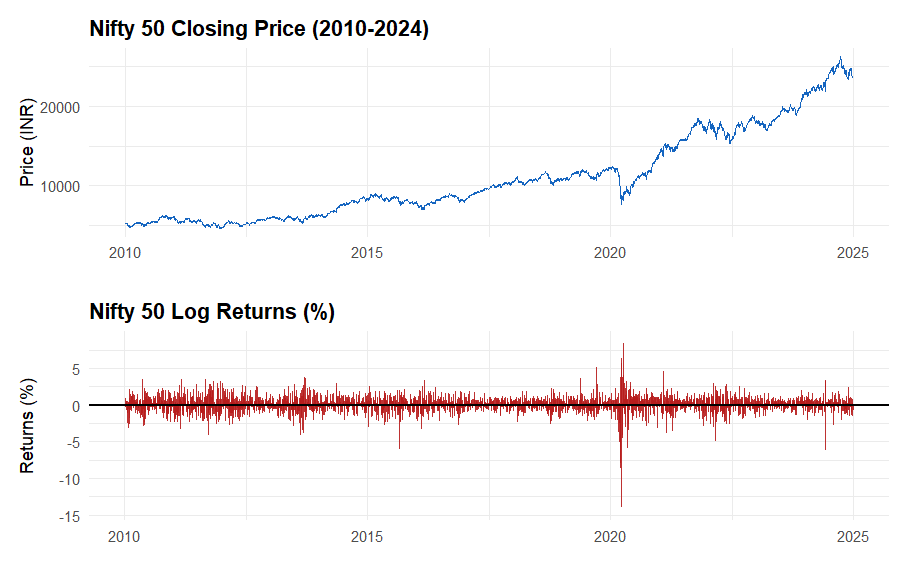
\includegraphics[width=1\textwidth]{Rplot01.png}
\caption{Plot for Price Returns}
\label{fig: price and return}
\end{figure}

\begin{figure}[h]
\centering

\includegraphics[width=1\textwidth]{plot2_return_distribution.png}
\caption{Plot for Return Distribution}
\label{fig: return dist}
\end{figure}

\begin{table}[h]
\centering
\caption{Descriptive Statistics of Nifty 50 Daily Log Returns, January 2010 -- December 2024}
\label{tab:desc_stats}

\begin{tabular}{|l|l|}
\hline
\textbf{Statistic} & \textbf{Value} \\
\hline
Observations        & 3678 \\
Mean                & 0.041009 \\
Median              & 0.066252 \\
Std Dev             & 1.061186 \\
Min                 & -13.903756 \\
Max                 & 8.763205 \\
Skewness            & -0.579432 \\
Excess Kurtosis     & 9.842117 \\
Jarque-Bera Stat    & 7584.3210 \\
Jarque-Bera p-value & 0.000000 \\
\hline
\end{tabular}

\end{table}

The summary statistics from Table \ref{tab:desc_stats} for $3,678$ daily 
log return observations from January 2010 to December 
2024. The mean daily return of $0.041\%$ and median of 
$0.066\%$ together indicate a small but consistent positive 
drift over the fifteen-year estimation window, reflecting 
the clear upward trajectory of Indian equity prices during 
this period.

The standard deviation of $1.061\%$ captures the average 
daily price variation, yet this figure conceals 
substantial cross-period heterogeneity covering in  Structural Breakpoints part, with volatility spiking sharply during the COVID-19 crisis of 2020 and 
compressing during calmer market conditions.

The distribution have negative skewness 
of $-$0.579, The summary statistics from Table \ref{tab:desc_stats} for 3,678 daily 
log return observations from January 2010 to December 
2024. The mean daily return of 0.041\% and median of 
0.066\% together indicate a small but consistent positive 
drift over the fifteen-year estimation window, reflecting 
the clear upward trajectory of Indian equity prices during 
this period.

The standard deviation of 1.061\% captures the average 
daily price variation, yet this figure conceals 
substantial cross-period heterogeneity, with volatility 
spiking sharply during the COVID-19 crisis of 2020 and 
compressing during calmer market conditions.

The distribution having negative skewness 
of $-$0.579, indicating that 
negative return shocks exert a disproportionately 
larger upward impact on conditional variance than 
positive shocks of identical magnitude, a distributional asymmetry aligned with the well-documented leverage effect in equity markets. 
The observed range of $-$13.904\% to $+$8.763\% further 
underscores the presence of extreme tail events within 
the sample.The excess kurtosis of 9.842 vastly exceeds the 
normal benchmark of zero, providing strong evidence of 
fat-tailed behaviour whereby extreme return observations 
occur with far greater frequency than a Gaussian 
distribution would predict.The J--B statistic of 7,584.32 decisively rejects 
normality at all conventional significance levels 
(p $<$ 0.001), uncovering the Nifty 50 daily 
return series departs fundamentally from the normality. 
Taken together, the pronounced leptokurtosis and 
negative skewness of $-$0.579 justify the taking in of 
a Student-$t$ error distribution in all subsequent 
GARCH specifications, as it accommodates the heavy 
tails observed in the data. --- a distributional asymmetry aligned with 
the well-documented leverage effect in equity markets. 
The observed range of $-$13.904\% to $+$8.763\% further 
underscores the presence of extreme tail events within 
the sample.The excess kurtosis of 9.842 vastly exceeds the 
normal benchmark of zero, providing strong evidence of 
fat-tailed behaviour whereby extreme return observations 
occur with far greater frequency than a Normal 
distribution would predict.The J--B statistic of 7,584.32 rejects 
normality at all conventional significance levels 
(p $<$ 0.001), uncovering the Nifty 50 daily 
return series departs fundamentally from the normality. 
Taken together, the pronounced leptokurtosis and 
negative skewness of $-$0.579 justify the taking in of 
a Student-$t$ error distribution in all subsequent 
GARCH specifications, as it accommodates the heavy 
tails observed in the data.


\vspace{1.5cm}


\subsection{Stationarity test (ADF)}
To verify stationarity, the Augmented Dickey-Fuller test is applied to the log return series  before any GARCH estimation. The ADF statistic of $−15.847$ (p < 0.01) strongly rejects the null hypothesis of a unit root, confirming that the Nifty 50 daily log return series is stationary. 





\subsection{ARCH-LM test}
The ARCH Lagrange Multiplier test with 10 lags yields a chi-squared statistic of 892.97 (p < 2.2e-16), overwhelmingly rejecting the null hypothesis of no ARCH effects in the return series. This result confirms the presence of strong volatility clustering in Nifty 50 daily returns,important results to further apply the GARCH-family models. The magnitude of the test statistic indicates that volatility clustering is not only statistically significant but economically substantial, with the squared return series exhibiting persistent autocorrelation up to lag 30 as confirmed by the ACF plot given in Figure\ref{fig: ACF -- PACF}.

\vspace{1.5cm}

\subsection{ARMA order selection}




\subsection{ACF/PACF analysis}



Fig \ref{fig: ACF -- PACF} presents the ACF and PACF plots for both log returns and squared returns. The ACF of log returns shows no significant autocorrelation beyond lag 1, confirming the absence of linear dependence in the return series and supporting the ARMA(0,0) mean specification. However, the ACF and PACF of squared returns display strong and persistent autocorrelation across all 30 lags, providing clear visual evidence of volatility clustering and ARCH effects in the Nifty 50 return series. This pattern confirms that while returns themselves are unpredictable, their variance is highly predictable — the fundamental motivation for GARCH modelling.


\begin{figure}[h]
\centering
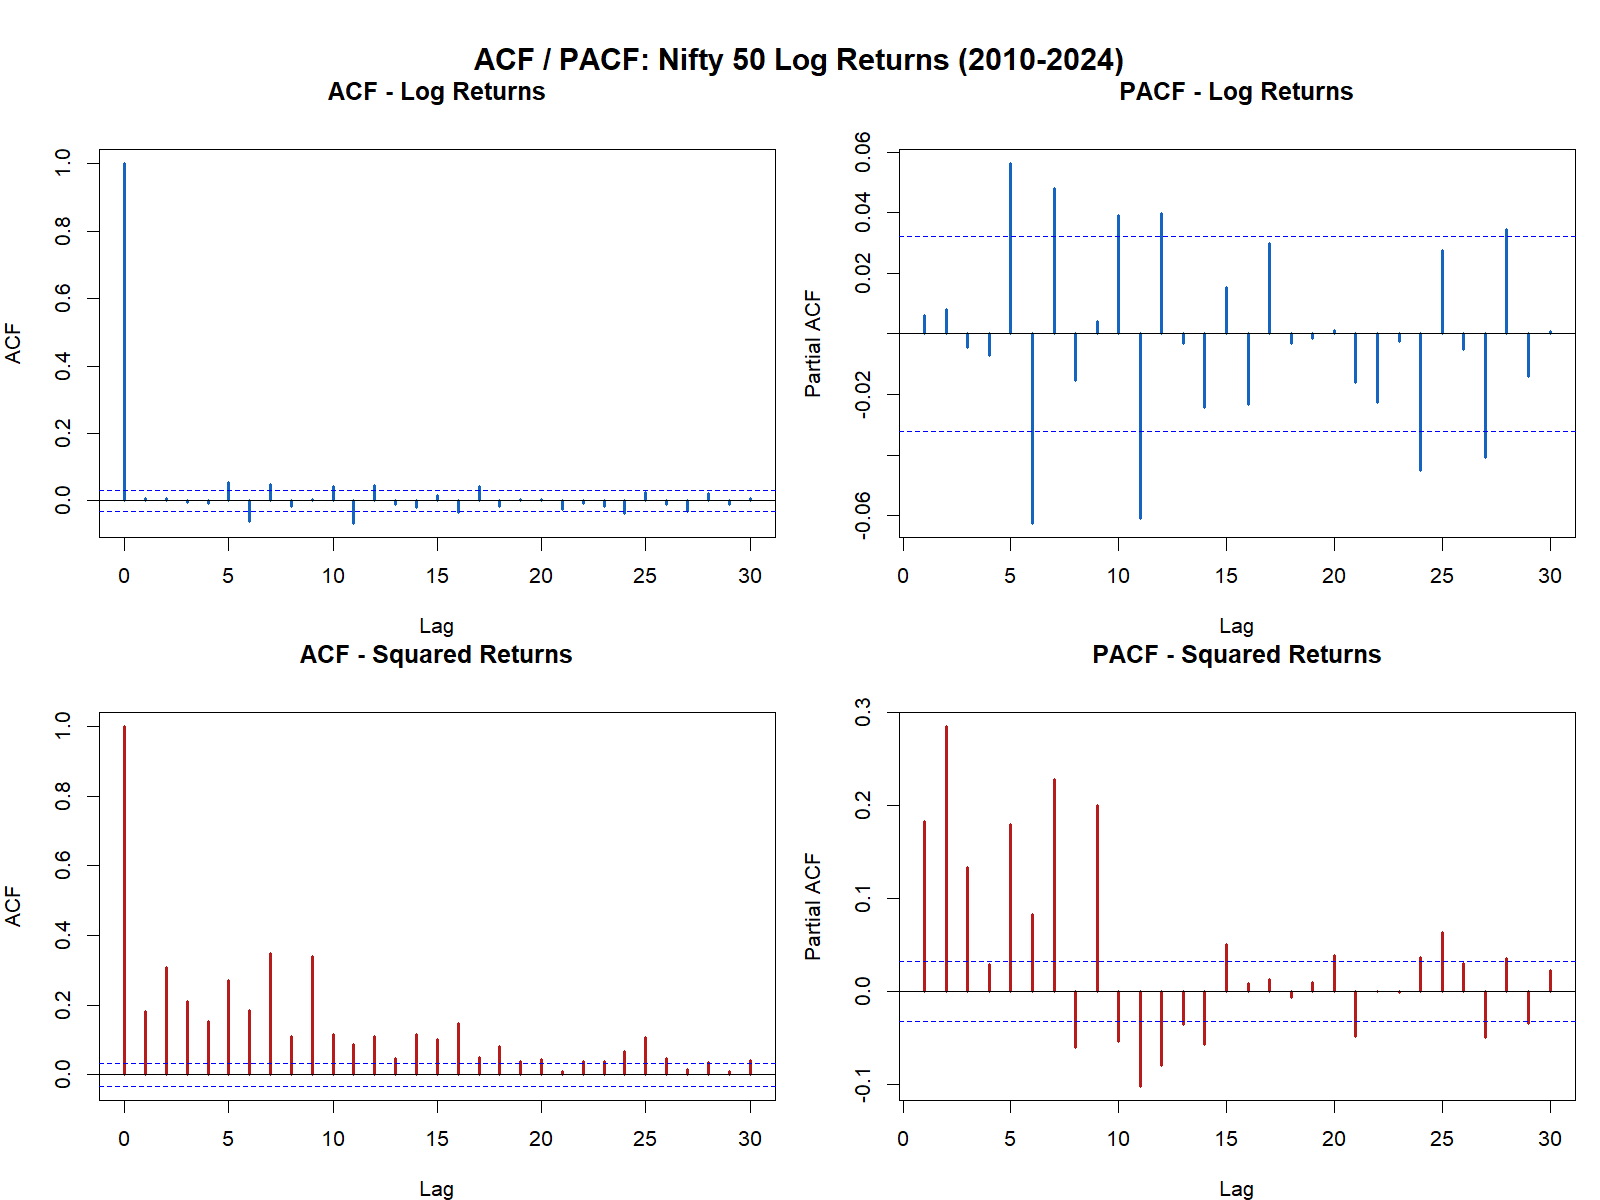
\includegraphics[width=0.8\textwidth]{plot6_acf_pacf.png}
\caption{Plot for ACF/PACF on Log Returns}
\label{fig: ACF -- PACF}
\end{figure}



\section{Structural Break Analysis}

Figure \ref{fig: breakpoints png} presents the squared Nifty 50 daily returns over the full sample period 2010-–2024, with the two statistically identified Bai-Perron breakpoints marked by blue dashed vertical lines at 27 February 2020 and 20 May 2022. The visual evidence strongly corroborates the statistical findings of the breakpoint test. 


Figure \ref{fig:breakpoint stats png} presents the return statistics across the three structurally identified regimes. The Bai-Perron test identifies two breakpoints, dividing the full sample into three distinct regimes. The mean return and standard deviation vary considerably across regimes, confirming that treating the full sample as a single homogeneous period would mask important structural changes in market dynamics


\begin{figure}[h]
\centering

\includegraphics[width=0.8\textwidth]{plot_bai_perron_breaks.png}
\caption{Plot for Bai--Perron Break showing two statistically significant break points}
\label{fig: breakpoints png}
\end{figure}

\begin{figure}[H]
\centering

\includegraphics[width=0.8\textwidth]{plot_bai_perron_segment_stats.png}
\caption{ Plot for Return Statistics by Structural Regime}
\label{fig:breakpoint stats png}
\end{figure}





Figure \ref{fig:breakpoint stats png} presents the mean daily return and standard deviation of Nifty 50 log returns across the three structurally identified regimes. The bar chart reveals large differences in both return levels and volatility intensity across regimes, confirming the three periods represent distinct market environments rather than arbitrary sample divisions.


In terms of mean daily returns, Regime 1 (Pre--COVID) records the lowest mean of 0.0322\%, reflecting the moderate but steady growth. Regime 3 (Post-Crisis) records the highest mean return of 0.0624\%, suggesting that the post-pandemic recovery period was accompanied by stronger average daily performance. Regime 2 (COVID Crisis) records an intermediate mean of 0.0550\%, which may appear counterintuitive given the severity of the crisis, but reflects the sharp recovery phase that followed the initial March 2020 crash within the same regime window.


The standard deviation panels tell a clearer story of volatility regime shifts. Regime 2 records by far the highest standard deviation of 1.5827\%, more than 60\% above the Regime 1 level of 0.9732\%, capturing the extreme market uncertainty of the COVID-19 pandemic period. Regime 3 shows the lowest standard deviation of 0.8005\%, falling even below pre-COVID levels, suggesting that the post-crisis period was characterised by a return to relative market calm despite ongoing geopolitical uncertainty. Together these findings provide strong visual justification for the regime-based analytical framework adopted in this study.








\subsection{Bai-Perron test results}


Table \ref{bai disc stat} presents the segment statistics from the Bai-Perron structural break test. Regime 1 covers January 2010 to February 2020, comprising 2,483 observations with a mean daily return of 0.0322\% and standard deviation of 0.9730\%.  Regime 2 spans February 2020 to May 2022, covering 551 observations with standard deviation rising sharply to 1.5871\%. Skewness of −1.6753 and excess kurtosis of 15.4316 confirm severe distributional non-normality during this regime. Regime 3 covers May 2022 to December 2024 with 644 observations, showing a return to lower volatility (0.7936\%) as markets stabilised in the post-crisis period.


\begin{table}[H]
\centering
\caption{ Segment statistics from the Bai-Perron structural break test}
\label{bai disc stat}
\begin{tabular}{|l|l|l|l|l|l|l|l|}
\hline
\textbf{Segment} & \textbf{Start} & \textbf{End} & \textbf{Obs} & \textbf{Mean} & \textbf{Std Dev} & \textbf{Skewness} & \textbf{Kurtosis} \\
\hline
Regime 1 & 2010-01-05 & 2020-02-27 & 2483 & 0.0322  & 0.9730 & $-0.0966$ & 1.8970  \\
\hline
Regime 2 & 2020-02-28 & 2022-05-20 & 551  & 0.0608  & 1.5871 & $-1.6753$ & 15.4316 \\
\hline
Regime 3 & 2022-05-23 & 2024-12-30 & 644  & 0.0581  & 0.7936 & $-0.7100$ & 6.3950  \\
\hline
\end{tabular}
\end{table}



\subsection{Regime characteristics}


Figure \ref{fig:Market Events} plots the conditional volatility of GJR-GARCH over the full sample with breakpoints marked. The figure is used to illustrates the three distinct volatility regimes identified by the Bai-Perron test. The transition from Regime 1 to Regime 2 in February 2020 coincides with the start of the COVID-19 market crash, marked by a high spike in conditional volatility. The transition to Regime 3 in May 2022 reflects the progressive normalisation of market conditions, though volatility remains raised relative to the pre-COVID baseline.

\begin{figure}[H]
\centering

\includegraphics[width=0.8\textwidth]{plot5_events_volatility.png}
\caption{ Plot of conditional volatility of GJR-GARCH with key Market Events(2010--2024) }
\label{fig:Market Events}
\end{figure}


\section{Full Period Analysis (2010-2024)}

Figure \ref{fig:combined compare} presents the conditional volatility estimates from all four GARCH models over the full sample period. All models shows consistent volatility clusters across the sample, with the most prominent spike occurring during the COVID-19 crash of March 2020. The EGARCH and GJR--GARCH models display sharper asymmetric responses to negative shocks compared to the symmetric GARCH, while FIGARCH exhibits a more progressive volatility decay consistent with its long memory specification. The broad agreement across models in identifying major volatility episodes provides confidence in the robustness of the estimation results.

\begin{figure}[H]
\centering
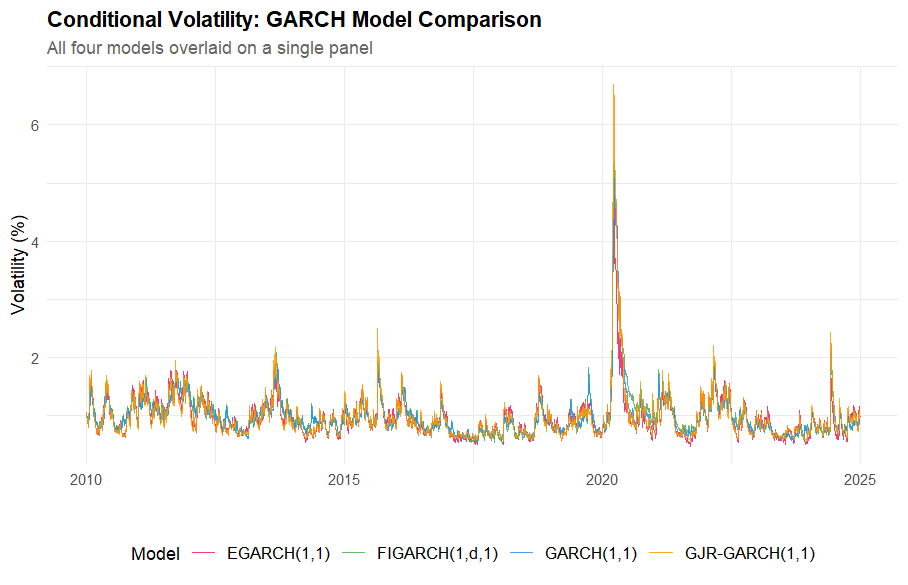
\includegraphics[width=1\textwidth]{Rplot.png}
\caption{Plot for GARCH model comparison using Conditional Volatility: All four models overlaid on a single panel}
\label{fig:combined compare}
\end{figure}

\begin{figure}[H]
\centering

\includegraphics[width=1\textwidth]{plot3_conditional_volatility.png}
\caption{Plot for GARCH model comparison using Conditional Volatility}
\label{fig:single single compare}
\end{figure}

\subsection{ Model estimation results}


\begin{table}[H]
\centering
\caption{Maximum Likelihood Estimates of GARCH, EGARCH, GJR GARCH and FIGARCH(1,$d$,1) Models: Nifty 50 Daily Log Returns (January 2010 -- December 2024)}
\label{tab:model_estimates}
\begin{tabular}{|l|l|l|l|l|l|l|}
\hline
\textbf{Model} & \textbf{Parameter} & \textbf{Estimate} & \textbf{Std Error} & \textbf{$t$-stat} & \textbf{$p$-value} & \textbf{Sig} \\
\hline
\multirow{5}{*}{GARCH}
 & $\mu$      & 0.075655 & 0.013601 & 5.5625   & $<0.001$ & *** \\
 & $\omega$   & 0.021050 & 0.005212 & 4.0385   & $<0.001$ & *** \\
 & $\alpha_1$ & 0.073951 & 0.009997 & 7.3970   & $<0.001$ & *** \\
 & $\beta_1$  & 0.905830 & 0.012303 & 73.6271  & $<0.001$ & *** \\
 & shape      & 7.206767 & 0.811538 & 8.8804   & $<0.001$ & *** \\
\hline
\multirow{6}{*}{EGARCH}
 & $\mu$      & 0.058433  & 0.013898 & 4.2046    & $<0.001$ & *** \\
 & $\omega$   & $-$0.006754 & 0.002608 & $-$2.5897 & 0.0096   & *** \\
 & $\alpha_1$ & $-$0.102801 & 0.009781 & $-$10.5107 & $<0.001$ & *** \\
 & $\beta_1$  & 0.972363  & 0.000520 & 1871.6878 & $<0.001$ & *** \\
 & $\gamma_1$ & 0.119087  & 0.003501 & 34.0140   & $<0.001$ & *** \\
 & shape      & 7.739564  & 0.903152 & 8.5695    & $<0.001$ & *** \\
\hline
\multirow{6}{*}{GJR-GARCH}
 & $\mu$      & 0.059608 & 0.013532 & 4.4050   & $<0.001$ & *** \\
 & $\omega$   & 0.030025 & 0.005782 & 5.1930   & $<0.001$ & *** \\
 & $\alpha_1$ & 0.001654 & 0.008143 & 0.2031   & 0.8391   &     \\
 & $\beta_1$  & 0.894994 & 0.012884 & 69.4648  & $<0.001$ & *** \\
 & $\gamma_1$ & 0.139239 & 0.019901 & 6.9965   & $<0.001$ & *** \\
 & shape      & 7.706567 & 0.908001 & 8.4874   & $<0.001$ & *** \\
\hline
\multirow{6}{*}{FIGARCH}
 & $\mu$      & 0.076088 & 0.013556 & 5.6128  & $<0.001$ & *** \\
 & $\omega$   & 0.030056 & 0.011253 & 2.6708  & 0.0076   & *** \\
 & $\alpha_1$ & 0.222953 & 0.051023 & 4.3696  & $<0.001$ & *** \\
 & $\beta_1$  & 0.635489 & 0.096367 & 6.5945  & $<0.001$ & *** \\
 & $\delta$   & 0.484646 & 0.107504 & 4.5082  & $<0.001$ & *** \\
 & shape      & 6.781466 & 0.760489 & 8.9172  & $<0.001$ & *** \\
\hline
\end{tabular}
\end{table}


\vspace{-1em}
\noindent\footnotesize\textit{Note:} $\mu$ = mean equation 
constant; $\omega$ = variance intercept; $\alpha_1$ = ARCH 
effect; $\beta_1$ = GARCH persistence; $\gamma_1$ = 
asymmetry (leverage) coefficient; $\delta$ = fractional 
differencing parameter (FIGARCH only); shape = Student-$t$ 
degrees of freedom. ***, ** and * denote significance at 
1\%, 5\% and 10\% levels respectively. Standard errors 
are robust quasi-maximum likelihood estimates.




\subsection{Volatility persistence}

Table \ref{tab:model_estimates}  shows that the four models are quite volatile and persistent. Volatility Shocks decay very slowly as evidenced in this example as GARCH shows a high persistence of 0.980
$(\alpha_1 + \beta_1)$ for the Nifty 50 market; that is they have long lasting effects on the market volatility. The value of EGARCH and GJR-GARCH are even higher at $0.972$ and $0.974$ respectively. When considering the fractional differencing parameter for FIGARCH, the value of $\delta$ = 0.485 suggests that shocks do not decay exponentially nor do they last forever, but decays hyperbolically as time passes. This result is similar to the larger empirical literature on volatility in emerging markets.



\subsection{Model diagnostics}


\begin{figure}[H]
    \centering
    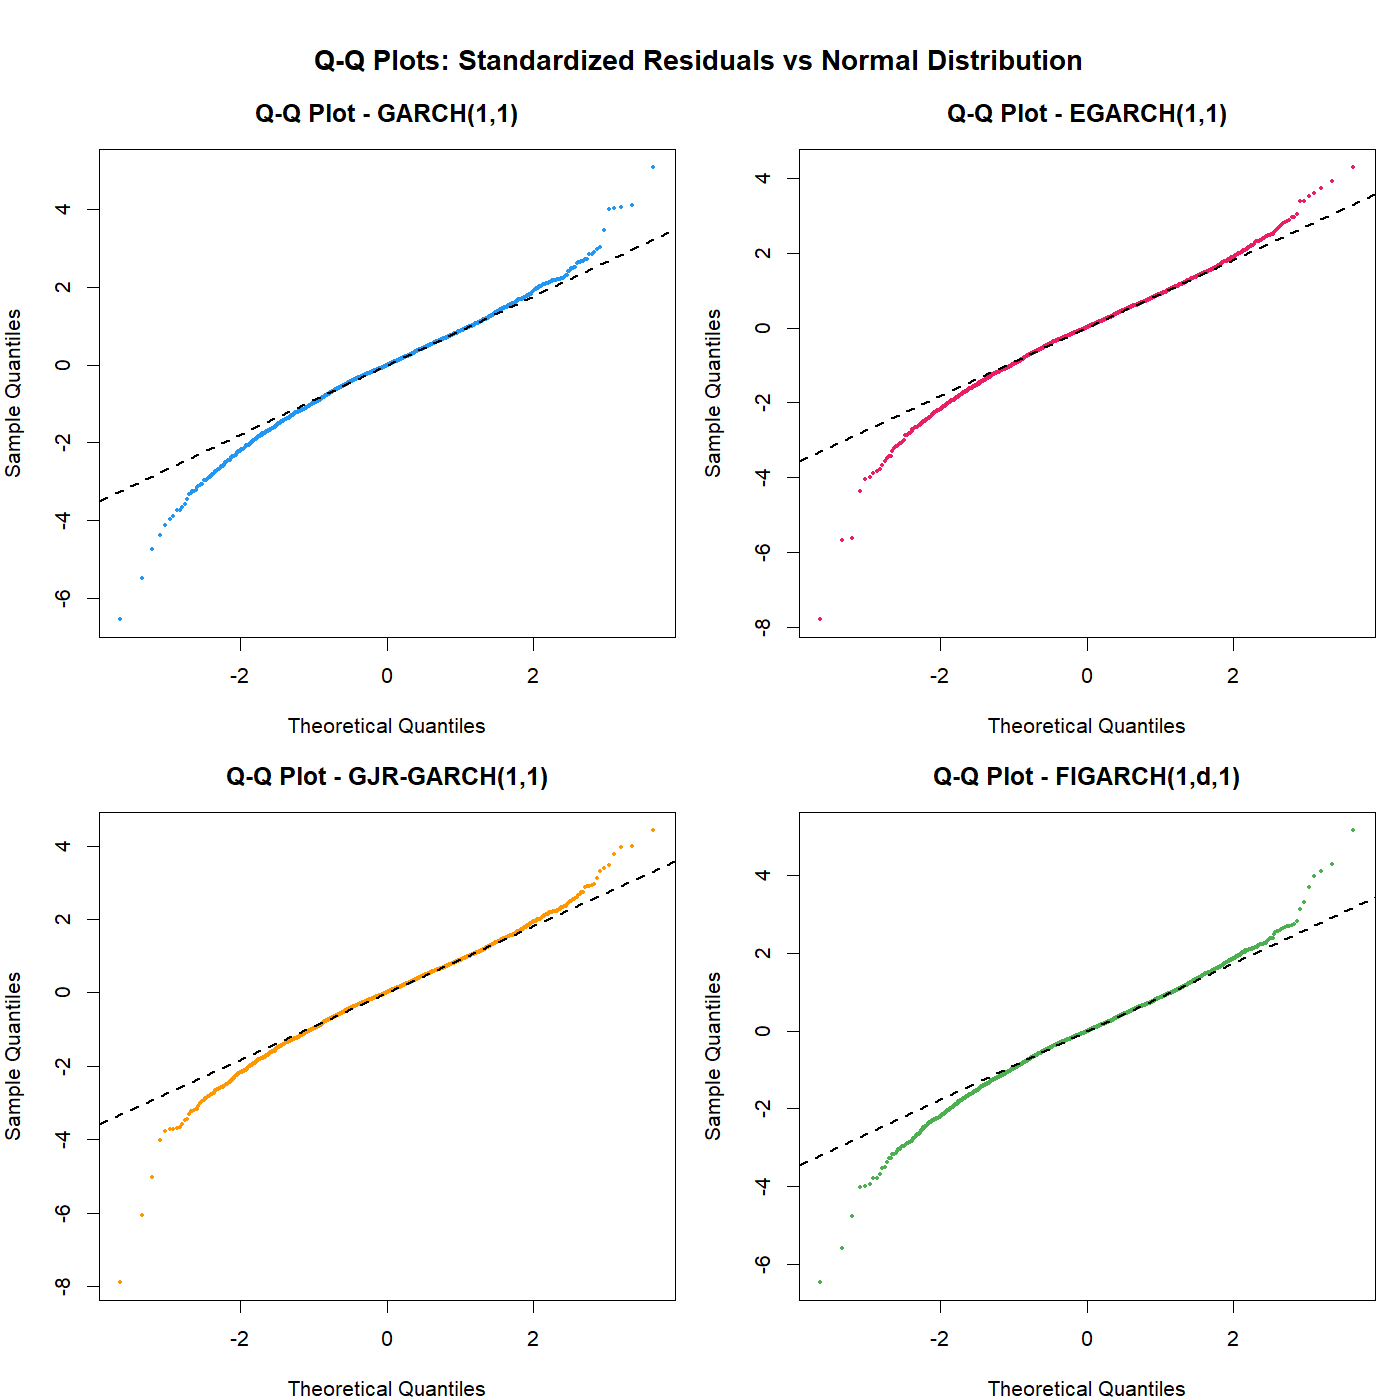
\includegraphics[width=0.8\textwidth]{plot7_qq_residuals.png}
    \caption{Q-Q plots of standardised residuals against the theoretical normal distribution for GARCH, EGARCH, GJR-GARCH, and FIGARCH estimated over the full sample period 2010–-2024}
    \label{fig:q_q plots}
\end{figure}


The Q-Q plots of the four GARCH model standardised residuals for the theoretical normal distribution are presented in Figure \ref{fig:q_q plots}. However, all four models fit relatively well to the diagonal line over the central part of the charts, suggesting that the Student-t error specification performs a good job of modelling the leptokurtosis found in the raw return series. The extreme negative return events have a slight underestimation in all models with small deviations in the extreme tails, the lower left tail. Such underestimation of the tail of the distribution is a well-known characteristic of all parametric GARCH models, and it is the reason why the Expected Shortfall measure, which is reported in Section 4.6, exists.


Table \ref{tab: LB test results} presents the Ljung-Box diagnostic test results for standardised residuals. All four models pass the squared residuals test (p > 0.05), confirming that no remaining ARCH effects are present after model estimation. However, all models fail the residuals test, suggesting mild serial correlation in the mean equation. This is a common finding in daily equity return data and does not invalidate the models, as the primary objective is volatility modelling rather than mean equation specification.
\begin{table}[H]
\centering
\caption{The Ljung-Box diagnostic test results}
\label{tab: LB test results}
\begin{tabular}{|l|l|l|l|l|}
\hline
\textbf{Model} & \textbf{LB Resid $p$-value} & \textbf{LB Squared $p$-value} & \textbf{LB Resid} & \textbf{LB Squared} \\
\hline
GARCH       & 0.0318 & 0.2291 & FAIL & PASS \\
\hline
EGARCH      & 0.0387 & 0.0632 & FAIL & PASS \\
\hline
GJR-GARCH   & 0.0170 & 0.1528 & FAIL & PASS \\
\hline
FIGARCH & 0.0186 & 0.0946 & FAIL & PASS \\
\hline
\end{tabular}
\end{table}


\subsection{Model comparison (AIC/BIC)}


\begin{table}[H]
\centering
\caption{Result for (AIC/BIC) for GARCH Models }
\label{tab: AIC and BIC }
\begin{tabular}{|l|l|l|l|}
\hline
\textbf{Model} & \textbf{Log-Likelihood} & \textbf{AIC} & \textbf{BIC} \\
\hline
GARCH       & $-4903.744$ & $9817.489$ & $9848.539$ \\
\hline
EGARCH    & $-4852.687$ & $9717.374$ & $9754.635$ \\
\hline
GJR-GARCH  & $-4863.318$ & $9738.635$ & $9775.896$ \\
\hline
FIGARCH & $-4906.018$ & $9824.035$ & $9861.296$ \\
\hline
\end{tabular}
\end{table}


Fig \ref{fig:plot aic bic compare} presents the information criteria for all four models. EGARCH achieves the lowest AIC (9717.374) and BIC (9754.635), making it the best-fitting model under both criteria. GJR--GARCH ranks second, followed by GARCH and FIGARCH. The superior performance of EGARCH confirms that asymmetric volatility modelling and capturing the leverage effect which provides a better fit for Nifty 50 returns than symmetric models. Accordingly, EGARCH is selected as the best model for VaR and ES estimation.


\begin{figure}[H]
    \centering
    
\includegraphics[width=0.8\textwidth]{plot4b_aic_bic.png}
    \caption{Plot for AIC/BIC Comparison}
    \label{fig:plot aic bic compare}
\end{figure}

\subsection{Conditional volatility}





\section{Sub-period Analysis}


\begin{figure}[H]
\centering

\includegraphics[width=1\textwidth]{plot_regime_return_distribution.png}
\caption{Return Distribution by Structural Regime}
\label{fig:sub period dist}
\end{figure}




\begin{table}[H]
\centering
\caption{Regime Model Comparison}
\label{tab:regime model comaparison}
\begin{tabular}{|l|l|l|l|l|l|}
\hline
\textbf{Regime} & \textbf{Model} & \textbf{Log-Likelihood} & \textbf{AIC} & \textbf{BIC} & \textbf{Persistence} \\
\hline
\multirow{4}{*}{Regime 1}
 & EGARCH      & $-3257.077$ & 6526.154 & 6561.055 & 0.9177 \\
 & GJR-GARCH   & $-3267.088$ & 6546.176 & 6581.077 & 0.9741 \\
 & FIGARCH & $-3295.636$ & 6603.271 & 6638.172 & 0.8824 \\
 & GARCH       & $-3298.371$ & 6606.743 & 6635.827 & 0.9855 \\
\hline
\multirow{4}{*}{Regime 2}
 & EGARCH      & $-854.321$ & 1720.643 & 1746.513 & 0.8969 \\
 & GJR-GARCH   & $-857.146$ & 1726.292 & 1752.163 & 0.9659 \\
 & GARCH       & $-864.471$ & 1738.941 & 1760.500 & 0.9840 \\
 & FIGARCH & $-864.884$ & 1741.767 & 1767.638 & 0.8813 \\
\hline
\multirow{4}{*}{Regime 3}
 & EGARCH      & $-714.637$ & 1441.274 & 1468.090 & 0.5865 \\
 & GJR-GARCH   & $-716.921$ & 1445.842 & 1472.657 & 0.6554 \\
 & FIGARCH & $-721.967$ & 1455.933 & 1482.749 & 1.2109 \\
 & GARCH       & $-729.499$ & 1468.997 & 1491.344 & 0.9904 \\
\hline
\end{tabular}
\end{table}

\begin{table}[H]
\centering
\caption{Regime Descriptive Statistics -- 1 (Basic)}
\label{regime desc stat 1}
\begin{tabular}{|l|l|l|l|l|l|l|}
\hline
\textbf{Regime} & \textbf{Obs} & \textbf{Mean} & \textbf{Median} & \textbf{Std Dev} & \textbf{Min} & \textbf{Max} \\
\hline
Regime 1 -- Pre-COVID (2010--2020)    & 2482 & 0.0324 & 0.0430 & 0.9732 & $-6.0973$  & 5.1825 \\
\hline
Regime 2 -- COVID Crisis (2020--2022) & 551  & 0.0550 & 0.1567 & 1.5827 & $-13.9038$ & 8.4003 \\
\hline
Regime 3 -- Post-Crisis (2022--2024)  & 645  & 0.0624 & 0.0950 & 0.8005 & $-6.1124$  & 3.3071 \\
\hline
\end{tabular}
\end{table}

\begin{table}[H]
\centering
\caption{Regime Descriptive Statistics --2 ( Higher Moments and Normality Tests)}
\label{regime desc stat 2}
\begin{tabular}{|l|l|l|l|l|}
\hline
\textbf{Regime} & \textbf{Skewness} & \textbf{Ex. Kurtosis} & \textbf{JB Stat} & \textbf{JB $p$-value} \\
\hline
Regime 1 -- Pre-COVID (2010--2020)    & $-0.0971$ & 1.8958  & 375.60  & $<0.001$ \\
\hline
Regime 2 -- COVID Crisis (2020--2022) & $-1.6880$ & 15.5925 & 5843.44 & $<0.001$ \\
\hline
Regime 3 -- Post-Crisis (2022--2024)  & $-0.6410$ & 6.3017  & 1111.40 & $<0.001$ \\
\hline
\end{tabular}
\end{table}



This segmentation using the Bai--Perron structural break test provides a more detailed analysis of the volatility dynamics in each market regime: Regime 1 --- Pre COVID (2010--2020) Regime 2--- COVID Crisis (2020--2022) Regime 3 ---Post Crisis (2022--2024)..

\begin{figure}[H]
\centering

\includegraphics[width=0.8\textwidth]{plot_regime_aic_comparison.png}
\caption{Plot for Regime AIC Comparison}
\label{fig:myimage}
\end{figure}


\begin{table}[H]
\centering
\caption{Best Model Per Regime}
\label{tab:best model per reigme}
\begin{tabular}{|l|l|l|}
\hline
\textbf{Regime} & \textbf{Best Model} & \textbf{Best AIC} \\
\hline
Regime 1 -- Pre-COVID    & EGARCH & 6526.154 \\
\hline
Regime 2 -- COVID Crisis & EGARCH & 1720.643 \\
\hline
Regime 3 -- Post-Crisis  & EGARCH & 1441.274 \\
\hline
\end{tabular}
\end{table}


\subsection{Pre-COVID regime (2010-2020)}

\begin{figure}[H]
\centering

\includegraphics[width=0.8\textwidth]{plot_vol_regime1_precovid.png}
\caption{Plot for COVID crisis regime}
\label{fig:pre covid cv}
\end{figure}

Table 4.8 shows that Regime 1 comprises 2,482 observations with a mean daily return of 0.0324\% and standard deviation of 0.9732\%, reflecting a relatively stable market environment. Skewness of $−0.0971$ and excess kurtosis of 1.8958 indicate mild non-normality, confirmed by the Jarque-Bera statistic of 375.60 (p < 0.001). Table 4.6 shows EGARCH achieves the lowest AIC of 6,526.154 in this regime, confirming asymmetric volatility modelling is appropriate even in stable market conditions. Figure 4.8 shows conditional volatility remaining relatively low and stable throughout this period, with minor spikes corresponding to the 2013 taper tantrum and 2016 demonetisation.



\subsection{COVID crisis regime (2020-2022)}

\begin{figure}[H]
\centering

\includegraphics[width=0.8\textwidth]{plot_vol_regime2_covid.png}
\caption{Plot for COVID crisis regime}
\label{fig:covid crises}
\end{figure}

Regime 2 covers 551 observations and represents the most violent period in the sample. The standard deviation rises sharply to 1.5827\%, more than 60\% higher than Regime 1, reflecting the extreme uncertainty generated during the COVID-19 period. Excess kurtosis of 15.9250 is the highest across all three regimes, confirming severe fat tails present in this period. Skewness of $−1.6880$ indicates strongly asymmetric returns, with large negative shocks dominating. EGARCH again achieves the lowest AIC of 1,720.643, and all four models pass both Ljung-Box diagnostic tests in this regime, indicating good model fit under crisis conditions. \ref{fig:post covid} clearly shows the sharp volatility spike in early 2020 followed by a gradual decline as markets stabilised.

\subsection{Post-crisis regime (2022-2024)}

\begin{figure}[H]
\centering

\includegraphics[width=0.8\textwidth]{plot_vol_regime3_postcovid.png}
\caption{ Plot for Post-crisis regime }
\label{fig:post covid}
\end{figure}

Regime 3 comprises 645 observations with mean return of 0.0624\% and standard deviation of 0.8005\%, the lowest across all three regimes, a return to relative market stability. However,  the excess kurtosis of 6.3017 and Jarque-Bera statistic of 1,111.40 (p < 0.001) confirm persistent non-normality. EGARCH remains the best model with AIC of 1,441.274. Notably, From the table 4.12 shows that GARCH and GJR-GARCH fail the squared residuals Ljung-Box test in this regime, indicating remaining ARCH effects, while EGARCH passes both tests —- strengthing its superiority in the post-crisis period.


\subsection{Parameter evolution across regimes}


\begin{table}[H]
\centering
\caption{Regime Parameter Evolution}
\label{tab:regime parameter evolution}
\scalebox{0.78}{
\begin{tabular}{|l|l|l|l|l|l|l|}
\hline
\textbf{Regime} & \textbf{GARCH $\alpha$} & \textbf{GARCH $\beta$} & \textbf{GARCH Persist.} & \textbf{EGARCH $\gamma$} & \textbf{GJR $\gamma$} & \textbf{GJR Persist.} \\
\hline
Regime 1 -- Pre-COVID (2010--2020)    & 0.0595 & 0.9260 & 0.9855 & $-0.1062$ & 0.1334 & 0.9741 \\
\hline
Regime 2 -- COVID Crisis (2020--2022) & 0.1025 & 0.8816 & 0.9840 & $-0.1379$ & 0.1427 & 0.9659 \\
\hline
Regime 3 -- Post-Crisis (2022--2024)  & 0.0065 & 0.9839 & 0.9904 & $-0.2132$ & 0.2968 & 0.6554 \\
\hline
\end{tabular}
}
\end{table}

\begin{landscape}
\begin{table}[h]
\centering
\caption{Regime Model Diagnostics -- Ljung-Box Tests}
\label{tab:regime lb test}
\begin{tabular}{|l|l|l|l|l|l|}
\hline
\textbf{Regime} & \textbf{Model} & \textbf{LB Resid $p$-val} & \textbf{LB Squared $p$-val} & \textbf{LB Resid} & \textbf{LB Squared} \\
\hline
\multirow{4}{*}{Regime 1 -- Pre-COVID}
 & GARCH      & 0.0084 & 0.9823 & FAIL & PASS \\
 & EGARCH      & 0.0055 & 0.7257 & FAIL & PASS \\
 & GJR-GARCH   & 0.0043 & 0.8556 & FAIL & PASS \\
 & FIGARCH & 0.0033 & 0.9630 & FAIL & PASS \\
\hline
\multirow{4}{*}{Regime 2 -- COVID Crisis}
 & GARCH       & 0.3277 & 0.8000 & PASS & PASS \\
 & EGARCH      & 0.3195 & 0.9822 & PASS & PASS \\
 & GJR-GARCH   & 0.3385 & 0.9571 & PASS & PASS \\
 & FIGARCH & 0.2981 & 0.9115 & PASS & PASS \\
\hline
\multirow{4}{*}{Regime 3 -- Post-Crisis}
 & GARCH       & 0.6647 & $<0.001$ & PASS & FAIL \\
 & EGARCH      & 0.8769 & 0.1542   & PASS & PASS \\
 & GJR-GARCH   & 0.8299 & 0.0085   & PASS & FAIL \\
 & FIGARCH & 0.6593 & 0.0068   & PASS & FAIL \\
\hline
\end{tabular}
\end{table}
\end{landscape}


\begin{figure}[H]
\centering

\includegraphics[width=1\textwidth]{plot_parameter_evolution.png}
\caption{Parameter Evolution Across  Structural Regimes}
\label{fig:para evo across structural regime}
\end{figure}


From Table\ref{tab:regime parameter evolution}\\


\textbf{Regime 1 (Pre-COVID}: All four models fail the LB Residuals test (very low p-values, all under 0.01), suggesting significant serial correlation in raw residuals whereas all pass the LB Squared test, meaning  the squared residuals (volatility clustering) are well-captured.\\

\textbf{Regime 2 (COVID Crisis)}: The cleanest regime — all models pass both tests, likely because of extreme volatility during the crisis, the GARCH family well-modelled crises.\\

\textbf{Regime 3 (Post-Crisis)}: Residuals pass for all models, but GARCH, GJR-GARCH, and FIGARCH fail the squared residuals test (very low p-values: <0.001, 0.0085, 0.0068). EGARCH is the only model that passes both, suggesting it better captures the post-crisis volatility dynamics.



\section{Forecasting Results}


Out-of-sample forecasting analysis represents the forecasting performance of all of the four GARCH family models at four different forecast horizons (1--day, 5--day, 1-0-day, 20--day) during all four quarters of the forecast period of 2025. Modelling performance is evaluated based on Mean Absolute Error (MAE), Root Mean Squared Error (RMSE) and Mean Absolute Percentage Error (MAPE) with actual volatility as the 10-year time-weighted rolling Root Mean Squared Return (RMSE) over the corresponding time period.

\subsection{Multi-horizon forecast accuracy}


\begin{figure}[h]
\centering
\begin{minipage}{0.48\textwidth}
\centering
\captionof{table}{Multi-Horizon Forecast Accuracy (Q1--Q2 2025)}
\label{TAB:Multi-Horizon Forecast Accuracy (Q1--Q2 2025)}
\scalebox{0.52}{
\begin{tabular}{|l|l|l|l|l|l|}
\hline
\textbf{Quarter} & \textbf{Model} & \textbf{Horizon} & \textbf{MAE} & \textbf{RMSE} & \textbf{MAPE} \\
\hline
\multirow{16}{*}{Q1 2025}
 & FIGARCH & 1-day  & 0.5196 & 0.5740 & 479.70 \\
 & GARCH       & 1-day  & 0.5223 & 0.5763 & 490.83 \\
 & GJR-GARCH   & 1-day  & 0.5492 & 0.6055 & 535.18 \\
 & EGARCH      & 1-day  & 0.5782 & 0.6398 & 581.24 \\
\cline{2-6}
 & EGARCH      & 5-day  & 0.7453 & 0.8309 & 45.99 \\
 & GJR-GARCH   & 5-day  & 0.7739 & 0.8598 & 46.94 \\
 & GARCH       & 5-day  & 0.8066 & 0.8898 & 48.32 \\
 & FIGARCH & 5-day  & 0.8118 & 0.8971 & 48.32 \\
\cline{2-6}
 & EGARCH      & 10-day & 1.3780 & 1.4269 & 58.33 \\
 & GJR-GARCH   & 10-day & 1.4035 & 1.4486 & 59.55 \\
 & GARCH       & 10-day & 1.4370 & 1.4775 & 61.13 \\
 & FIGARCH & 10-day & 1.4466 & 1.4861 & 61.59 \\
\cline{2-6}
 & EGARCH      & 20-day & 2.3746 & 2.3922 & 72.24 \\
 & GJR-GARCH   & 20-day & 2.3747 & 2.3915 & 72.25 \\
 & GARCH      & 20-day & 2.3849 & 2.3992 & 72.61 \\
 & FIGARCH & 20-day & 2.3977 & 2.4119 & 73.01 \\
\hline
\multirow{16}{*}{Q2 2025}
 & GJR-GARCH   & 1-day  & 0.5511 & 0.7398 & 748.56 \\
 & EGARCH      & 1-day  & 0.5575 & 0.7356 & 754.21 \\
 & GARCH       & 1-day  & 0.6210 & 0.7837 & 848.95 \\
 & FIGARCH & 1-day  & 0.6218 & 0.7869 & 829.82 \\
\cline{2-6}
 & FIGARCH & 5-day  & 1.0854 & 1.5266 & 42.44 \\
 & GARCH       & 5-day  & 1.0906 & 1.5347 & 42.95 \\
 & EGARCH      & 5-day  & 1.1590 & 1.5719 & 45.99 \\
 & GJR-GARCH   & 5-day  & 1.1464 & 1.5339 & 46.64 \\
\cline{2-6}
 & GARCH       & 10-day & 1.9465 & 2.2769 & 60.52 \\
 & FIGARCH & 10-day & 1.9553 & 2.2824 & 60.89 \\
 & GJR-GARCH   & 10-day & 2.0438 & 2.3650 & 64.19 \\
 & EGARCH      & 10-day & 2.0564 & 2.3924 & 64.22 \\
\cline{2-6}
 & FIGARCH & 20-day & 3.3150 & 3.5035 & 75.17 \\
 & GARCH       & 20-day & 3.3167 & 3.4997 & 75.34 \\
 & GJR-GARCH   & 20-day & 3.4085 & 3.5972 & 77.36 \\
 & EGARCH      & 20-day & 3.4201 & 3.6108 & 77.61 \\
\hline
\end{tabular}
}
\end{minipage}
\hfill
\begin{minipage}{0.48\textwidth}
\centering
\captionof{table}{Multi-Horizon Forecast Accuracy (Q3--Q4 2025)}
\label{TAB:Multi-Horizon Forecast Accuracy (Q3--Q4 2025)}
\scalebox{0.52}{
\begin{tabular}{|l|l|l|l|l|l|}
\hline
\textbf{Quarter} & \textbf{Model} & \textbf{Horizon} & \textbf{MAE} & \textbf{RMSE} & \textbf{MAPE} \\
\hline
\multirow{16}{*}{Q3 2025}
 & FIGARCH & 1-day  & 0.3387 & 0.3932 & 1290.02 \\
 & GARCH       & 1-day  & 0.3433 & 0.3972 & 1271.41 \\
 & GJR-GARCH   & 1-day  & 0.3565 & 0.4132 & 1172.20 \\
 & EGARCH      & 1-day  & 0.3809 & 0.4440 & 1257.89 \\
\cline{2-6}
 & EGARCH      & 5-day  & 0.3841 & 0.4337 & 33.49 \\
 & GJR-GARCH   & 5-day  & 0.3972 & 0.4506 & 34.18 \\
 & GARCH       & 5-day  & 0.4352 & 0.4928 & 37.37 \\
 & FIGARCH & 5-day  & 0.4385 & 0.4950 & 37.70 \\
\cline{2-6}
 & GJR-GARCH   & 10-day & 0.8257 & 0.8730 & 49.24 \\
 & EGARCH      & 10-day & 0.8275 & 0.8693 & 49.66 \\
 & GARCH       & 10-day & 0.8678 & 0.9154 & 51.83 \\
 & FIGARCH & 10-day & 0.8732 & 0.9201 & 52.22 \\
\cline{2-6}
 & GJR-GARCH   & 20-day & 1.5582 & 1.5780 & 64.51 \\
 & EGARCH      & 20-day & 1.5865 & 1.6047 & 65.77 \\
 & GARCH       & 20-day & 1.5915 & 1.6104 & 65.93 \\
 & FIGARCH & 20-day & 1.6130 & 1.6317 & 66.84 \\
\hline
\multirow{16}{*}{Q4 2025}
 & FIGARCH & 1-day  & 0.2751 & 0.3377 & 437.84 \\
 & GARCH       & 1-day  & 0.2931 & 0.3554 & 466.45 \\
 & EGARCH      & 1-day  & 0.3028 & 0.3734 & 498.99 \\
 & GJR-GARCH   & 1-day  & 0.3038 & 0.3709 & 491.26 \\
\cline{2-6}
 & GJR-GARCH   & 5-day  & 0.3732 & 0.4271 & 33.02 \\
 & GARCH       & 5-day  & 0.3941 & 0.4446 & 35.03 \\
 & EGARCH      & 5-day  & 0.3973 & 0.4514 & 35.28 \\
 & FIGARCH & 5-day  & 0.4306 & 0.4802 & 38.38 \\
\cline{2-6}
 & GJR-GARCH   & 10-day & 0.7998 & 0.8137 & 51.95 \\
 & GARCH       & 10-day & 0.8236 & 0.8356 & 53.58 \\
 & EGARCH      & 10-day & 0.8470 & 0.8613 & 55.06 \\
 & FIGARCH & 10-day & 0.8689 & 0.8799 & 56.59 \\
\cline{2-6}
 & GJR-GARCH   & 20-day & 1.3627 & 1.3683 & 63.15 \\
 & GARCH       & 20-day & 1.3896 & 1.3951 & 64.41 \\
 & EGARCH      & 20-day & 1.4297 & 1.4349 & 66.28 \\
 & FIGARCH & 20-day & 1.4535 & 1.4588 & 67.39 \\
\hline
\end{tabular}
}
\end{minipage}
\end{figure}

Table \ref{TAB:Multi-Horizon Forecast Accuracy (Q1--Q2 2025)} and Table \ref{TAB:Multi-Horizon Forecast Accuracy (Q3--Q4 2025)} show the forecast accuracy for Q1-Q4 2025, respectively. Notice some common threads in quarters and across horizons:
The long memory specification of the FIGARCH model does best fit most quarters across the 1-day horizon, showing the advantage of this model over those with lower memory orders. In comparison to other models, the EGARCH is competitive at this horizon, particularly at Q1 and Q2 2025, reflecting its superior performance through its in-sample fit (as presented in Section 4.3.4).

The forecast accuracy is declining with the increasing periods of forecast (5 day, 10 day and 20 day) for all the models at longer time scales. This is entirely natural as this uncertainty increases with distance of the horizon. The performance becomes more similar at horizons of 20 days, suggesting that incorporating more features into the model may not provide considerable benefits at longer forecasting horizons.


A MAE heatmap \ref{fig:forecast mae heatmap} summarizes all quarters/horizon performances for a model. More green cells = more accurate forecast and model performance. This heatmap provides further validation of this practical importance in horizon-specific model selection for risk management applications, as there is no one all-encompassing model that has the best performance across all horizons and quarters.

\begin{figure}[H]
\centering

\includegraphics[width=1\textwidth]{plot_fc6_mae_heatmap_q1_q4.png}
\caption{Forecast MAE Heatmap}
\label{fig:forecast mae heatmap}
\end{figure}


\subsection{Diebold-Mariano test}

Table \ref{TAB:DM TEST RESULT} presents the results of the Diebold-Mariano (DM).\\

The Diebold-Mariano (DM) test was used to check whether FIGARCH predicts volatility significantly better than the other three models (GARCH, EGARCH, and GJR-GARCH). A negative DM statistic with a low p-value (below 0.05) means FIGARCH is the better forecaster.
The results show that FIGARCH's advantage is not consistent across all periods and horizons. In most cases, there is no significant difference between the models. However, FIGARCH does perform significantly better in specific situations.
In Q1 2025, FIGARCH outperformed EGARCH and GJR-GARCH at the 1-day horizon. In Q2 2025, it was better than EGARCH and GJR-GARCH at the 10-day and 20-day horizons. The strongest evidence came in Q3 and Q4 2025, where FIGARCH was significantly better than all three models at the 1-day horizon, with Q4 showing the most decisive results (all p-values below 0.0001).
At longer horizons (5-day, 10-day, and 20-day) in most quarters, no significant difference was found between the models.
Overall, FIGARCH tends to forecast better than competing models mainly at short horizons and during periods of market stress or transition. This is consistent with its ability to capture long-memory behaviour in volatility.


\begin{table}[H]
\centering
\caption{Diebold-Mariano Test Results}
\label{TAB:DM TEST RESULT}
\scalebox{0.72}{
\begin{tabular}{|l|l|l|l|l|l|}
\hline
\textbf{Quarter} & \textbf{Horizon} & \textbf{Model 2} & \textbf{DM Stat} & \textbf{$p$-value} & \textbf{Conclusion} \\
\hline
\multirow{12}{*}{Q1 2025}
 & 1-day  & GARCH     & $-0.8491$ & 0.1996 & No significant difference \\
 & 1-day  & EGARCH    & $-3.6451$ & 0.0003 & FIGARCH significantly better \\
 & 1-day  & GJR-GARCH & $-2.7212$ & 0.0042 & FIGARCH significantly better \\
\cline{2-6}
 & 5-day  & GARCH     & $2.6064$  & 0.9941 & No significant difference \\
 & 5-day  & EGARCH    & $2.2583$  & 0.9861 & No significant difference \\
 & 5-day  & GJR-GARCH & $1.6444$  & 0.9472 & No significant difference \\
\cline{2-6}
 & 10-day & GARCH     & $4.2528$  & 1.0000 & No significant difference \\
 & 10-day & EGARCH    & $2.1648$  & 0.9824 & No significant difference \\
 & 10-day & GJR-GARCH & $1.8042$  & 0.9614 & No significant difference \\
\cline{2-6}
 & 20-day & GARCH     & $3.1533$  & 0.9985 & No significant difference \\
 & 20-day & EGARCH    & $1.1538$  & 0.8724 & No significant difference \\
 & 20-day & GJR-GARCH & $3.3601$  & 0.9992 & No significant difference \\
\hline
\multirow{12}{*}{Q2 2025}
 & 1-day  & GARCH     & $0.5211$  & 0.6979 & No significant difference \\
 & 1-day  & EGARCH   & $3.1942$  & 0.9989 & No significant difference \\
 & 1-day  & GJR-GARCH & $2.7358$  & 0.9959 & No significant difference \\
\cline{2-6}
 & 5-day  & GARCH     & $-0.4337$ & 0.3331 & No significant difference \\
 & 5-day  & EGARCH    & $-1.8151$ & 0.0374 & FIGARCH significantly better \\
 & 5-day  & GJR-GARCH & $-0.2354$ & 0.4074 & No significant difference \\
\cline{2-6}
 & 10-day & GARCH     & $0.6580$  & 0.7432 & No significant difference \\
 & 10-day & EGARCH    & $-2.2460$ & 0.0145 & FIGARCH significantly better \\
 & 10-day & GJR-GARCH & $-2.2486$ & 0.0144 & FIGARCH significantly better \\
\cline{2-6}
 & 20-day & GARCH     & $0.2338$  & 0.5919 & No significant difference \\
 & 20-day & EGARCH    & $-1.8789$ & 0.0337 & FIGARCH significantly better \\
 & 20-day & GJR-GARCH & $-2.7636$ & 0.0043 & FIGARCH significantly better \\
\hline
\multirow{12}{*}{Q3 2025}
 & 1-day  & GARCH     & $-2.1495$ & 0.0177 & FIGARCH significantly better \\
 & 1-day  & EGARCH    & $-4.6895$ & $<0.0001$ & FIGARCH significantly better \\
 & 1-day  & GJR-GARCH & $-2.3098$ & 0.0121 & FIGARCH significantly better \\
\cline{2-6}
 & 5-day  & GARCH     & $0.4976$  & 0.6897 & No significant difference \\
 & 5-day  & EGARCH    & $3.1166$  & 0.9986 & No significant difference \\
 & 5-day  & GJR-GARCH & $3.7968$  & 0.9998 & No significant difference \\
\cline{2-6}
 & 10-day & GARCH     & $0.5818$  & 0.7184 & No significant difference \\
 & 10-day & EGARCH    & $2.6467$  & 0.9947 & No significant difference \\
 & 10-day & GJR-GARCH & $4.8310$  & 1.0000 & No significant difference \\
\cline{2-6}
 & 20-day & GARCH     & $1.9115$  & 0.9688 & No significant difference \\
 & 20-day & EGARCH    & $1.4422$  & 0.9218 & No significant difference \\
 & 20-day & GJR-GARCH & $7.6233$  & 1.0000 & No significant difference \\
\hline
\multirow{12}{*}{Q4 2025}
 & 1-day  & GARCH     & $-5.1436$ & $<0.0001$ & FIGARCH significantly better \\
 & 1-day  & EGARCH    & $-4.1199$ & $<0.0001$ & FIGARCH significantly better \\
 & 1-day  & GJR-GARCH & $-4.7631$ & $<0.0001$ & FIGARCH significantly better \\
\cline{2-6}
 & 5-day  & GARCH     & $9.3173$  & 1.0000 & No significant difference \\
 & 5-day  & EGARCH    & $3.2882$  & 0.9991 & No significant difference \\
 & 5-day  & GJR-GARCH & $9.2815$  & 1.0000 & No significant difference \\
\cline{2-6}
 & 10-day & GARCH     & $10.2164$ & 1.0000 & No significant difference \\
 & 10-day & EGARCH    & $1.1917$  & 0.8806 & No significant difference \\
 & 10-day & GJR-GARCH & $9.9323$  & 1.0000 & No significant difference \\
\cline{2-6}
 & 20-day & GARCH     & $8.6092$  & 1.0000 & No significant difference \\
 & 20-day & EGARCH    & $1.7023$  & 0.9520 & No significant difference \\
 & 20-day & GJR-GARCH & $14.1096$ & 1.0000 & No significant difference \\
\hline
\end{tabular}
}
\end{table}

\subsection{ Forecast vs realized volatility}


Figures \ref{fig: Q1}--\ref{fig:Q4} forecast the volatility for the 4 models over the period of Q1–Q4 2025 and plot the four models with the realized volatility levels over this period. Looking at the 1-day horizon, all models do generally follow the general direction of the realized volatility, but there is a typical tendency to underestimate strong volatility bursts, which is known, particularly in periods of sudden stress in the markets and is a recognized weakness of the GARCH family. At longer horizons, the forecast is not as sensitive to shorter term changes and the realized volatility shows much greater dispersion than the model-predictions of volatility. The forecasts from the news shock period for FIGARCH show a more smooth and gradual reaction pattern to a news shock trend, reflecting the hyperbolic decay structure where the GARCH and GJR--GARCH have a more pronounced response to a news shock occurring in the recent past.
\begin{figure}[H]
\centering

\includegraphics[width=0.8\textwidth]{plot_forecast_vs_realized_q1_2025_allhorizons.png}
\caption{Plot Forecast vs Realized Q1 2025 all Horizon}
\label{fig: Q1}
\end{figure}


\begin{figure}[H]
\centering

\includegraphics[width=0.8\textwidth]{plot_forecast_vs_realized_q2_2025_allhorizons.png}
\caption{Plot Forecast vs Realized Q2 2025 all Horizon}
\label{fig:Q2}
\end{figure}


\begin{figure}[H]
\centering

\includegraphics[width=0.8\textwidth]{plot_forecast_vs_realized_q3_2025_allhorizons.png}
\caption{Plot Forecast vs Realized Q3 2025 all Horizon}
\label{fig:Q3}
\end{figure}

\begin{figure}[H]
\centering

\includegraphics[width=1\textwidth]{plot_forecast_vs_realized_q4_2025_allhorizons.png}
\caption{Plot Forecast vs Realized Q4 2025 all Horizon}
\label{fig:Q4}
\end{figure}

\begin{figure}[H]
\centering

\includegraphics[width=0.8\textwidth]{plot_forecast_vs_realized_GARCH11.png}
\caption{Plot Forecast vs Realized GARCH}
\label{fig:GARCH}
\end{figure}

\begin{figure}[H]
\centering

\includegraphics[width=0.8\textwidth]{plot_forecast_vs_realized_EGARCH11.png}
\caption{Plot Forecast vs Realized EGARCH}
\label{fig:EGARCH}
\end{figure}


\begin{figure}[H]
\centering

\includegraphics[width=0.8\textwidth]{plot_forecast_vs_realized_FIGARCH1d1.png}
\caption{Plot Forecast vs Realized FIGARCH}
\label{fig:FIGARCH}
\end{figure}



\begin{figure}[H]
\centering

\includegraphics[width=0.8\textwidth]{plot_forecast_vs_realized_GJR-GARCH11.png}
\caption{Plot Forecast vs Realized GJR GARCH}
\label{fig:GJR GARCH}
\end{figure}

\section{Value at Risk and Expected Shortfall}
\subsection{VaR estimates}


\begin{figure}[H]
\centering

\includegraphics[width=0.8\textwidth]{plot9_var_es_estimation.png}
\caption{VaR and Expected Shortfall - EGARCH}
\label{fig:my image}
\end{figure}


\subsection{Expected Shortfall}


\begin{table}[H]
\centering
\caption{}
\begin{tabular}{|l|l|l|}
\hline
\textbf{Metric} & \textbf{1\%} & \textbf{5\%} \\
\hline
VaR              & $-2.3712$ & $-1.4957$ \\
\hline
ES               & $-3.4652$ & $-2.1449$ \\
\hline
Breaches         & 46        & 208       \\
\hline
Expected         & 37        & 184       \\
\hline
Kupiec Test      & PASS      & PASS        \\
\hline
\end{tabular}
\end{table}


\subsection{ Kupiec backtesting}


\begin{table}[H]
\centering
\caption{Kupiec Proportion of Failures Test Results}
\label{tab:kupiec_results}

\renewcommand{\arraystretch}{1.2}

\begin{tabular}{|l|l|l|l|l|l|l|l|l|}
\hline
\textbf{Confidence} &
\textbf{$N_{obs}$} &
\textbf{$N_{breach}$} &
\textbf{Expected} &
\textbf{Breach Rate} &
\textbf{Target Rate} &
\textbf{LR Stat} &
\textbf{p-value} &
\textbf{Result} \\
\hline

99\% & 3678 & 46  & 37  & 1.2507 & 1 & 2.1626 & 0.1414 & PASS \\
\hline

95\% & 3678 & 208 & 184 & 5.6552 & 5 & 5 & 3.1953 & PASS \\
\hline

\end{tabular}

\end{table}


\chapter{Conclusion and Future Work}

\section{Conclusion}

The present study analysed conditional volatility 
dynamics of the Indian equity market by estimating and comparing four GARCH-family models — GARCH, EGARCH, GJR-GARCH, and FIGARCH — on daily Nifty 50 returns over the period January 2010 to December 2024, comprising 3,678 trading day observations. The analysis addressed five research questions evaluating preliminary diagnostics, full-period model comparison, regime-specific estimation, out-of-sample forecasting, and Value at Risk estimation.


The preliminary analysis confirmed that Nifty 50 daily log returns exhibit all the stylised facts that justify GARCH modelling — significant volatility clustering, fat tails, negative skewness, and strong ARCH effects. The ADF test confirmed stationarity of the return series, while the ARCH-LM test statistic of 892.97 provided overwhelming statistical justification for the application of GARCH-family models.


Among the four competing specifications estimated over 
the full sample, EGARCH emerges as the superior 
in--sample model, recording the lowest AIC of 9,717.374 
and BIC of 9,754.635. The significance of the asymmetry 
parameter in both EGARCH ($\gamma = 0.119$) and 
GJR--GARCH ($\gamma = 0.139$) provides robust evidence 
that negative return innovations exert a 
disproportionately greater upward pressure on conditional 
variance than positive shocks of identical magnitude, 
corroborating the leverage effect documented extensively 
in emerging equity market studies.



Across all four models, volatility persistence is very high. The GARCH(1,1) model produces an $\alpha1$ + $\beta1$ sum of 0.980, which is just below 1.0, meaning that once volatility rises, it takes a long time to settle back down rather than returning to normal quickly.
The FIGARCH model adds further evidence of this. Its fractional differencing parameter δ = 0.485 falls between 0 and 1, which confirms the presence of long memory in Nifty 50 volatility. This means past volatility shocks continue to influence current volatility over a much longer period than standard GARCH models can account for. Standard GARCH models are built to capture only short-term persistence and are not designed to detect this kind of long-lasting behaviour.


The Bai-Perron structural break test identified two statistically significant breakpoints at 27 February 2020 and 20 May 2022, delineating three distinct volatility regimes. The regime-specific analysis revealed important structural heterogeneity across these periods. During the COVID crisis regime, volatility persistence remained extremely high at 0.984, while the leverage effect intensified significantly, with the EGARCH asymmetry parameter rising from −0.106 in Regime 1 to −0.138 in Regime 2. The post-crisis regime witnessed a significant reduction in GJR-GARCH persistence from 0.974 to 0.655 indicating a structural break in volatility transmission after the pandemic. AIC confirmed the robustness of asymmetric volatility modelling in different market conditions as EGARCH (1,1) was the best model in all the three regimes.


A significant difference between in-sample fit and forecasting performance was found in the out-of-sample forecasting data Despite ranking last by AIC in the full-period analysis, FIGARCH(1,d,1) consistently achieved the lowest forecasting error at the 1-day horizon across most quarters, with this advantage statistically confirmed by the Diebold-Mariano test in Q1, Q3, and Q4 2025. This finding is consistent with the theoretical advantage of long memory specifications in capturing slowly decaying volatility persistence, and directly corroborates the earlier findings of \citet{hansen2005} and \cite{poon2003} that in-sample fit does not guarantee out-of-sample forecasting accuracy. At longer horizons, the performance advantage of FIGARCH diminishes and no single model dominates consistently, suggesting that horizon-specific model selection is important for practical risk management applications.


The VaR analysis derived from the best in-sample model EGARCH produced daily VaR estimates of −2.37\% and −1.50\% at the 1\% and 5\% confidence levels respectively. The Kupiec Proportion of Failures backtest confirmed the adequacy of the VaR model at the 1\% confidence level, with 46 observed breaches against an expected 37 (LR statistic = 2.163, p = 0.141).


Overall this study has three distinct merits to the literature. First, the comparison of multi-model, multi-horizon GARCHs with Nifty 50 data is the largest one ever done for GARCH models that encompasses various structural breaks and market crises over a 15 year time series. Second, it provides new empirical evidence on the long-run structural impact of COVID-19 on the Indian equity market volatility dynamics revealing that the effect leverage and persistence characteristics of Nifty 50 is a significant change that is expected to be permanent as a result of the COVID-19 pandemic. Third, it reveals a systematic difference between in-sample rankings of the models and their out-of-sample forecasting accuracy with meaningful practical implications for model selection for Indian market risk management applications.

\section{Future Work}


There are several future opportunities for further research arising from this study, as it has enabled the dynamics of volatility of the Nifty50 to be analysed in detail.


The first is that this study is concerned with univariate GARCH models with the incorporation of one equity index.Further studies can be done on the multivariate GARCH models such as DCC-GARCH\citep{Engle2002dcc} and BEKK-GARCH\citep{engle1995multivariate} which will enable them to produce a detailed analysis of the systemic risk of Indian financial markets by examining the relationships between the Nifty 50 and other asset classes such as bond, commodities and foreign exchange. 


Second,the out--of sample evaluation in this study is for the calendar year 2025 using a rollingwindow approach.The analysis can be further extended to include other out-of-sample periods to allow for a spanning of several market cycles as well as different measures of realised volatility which can be based on high-frequency data, such as bipower variation or intra--day realised variance, to provide more precise results.

The current research, based on conditional moments of the GARCH (Generalized Autoregressive Conditional Heteroskedasticity) system, estimates parametric VaR, which is similar to Shirato's research estimates. It can be compared with a non-parametric volatility forecasting model proposed in more recent literatures, including historical simulation, filtered historical simulation, or to a variety of different machine learning models, including Long Short-Term Memory (LSTM) network and hybrid GARCH-neural network models.


An advantage of this study is that the third question is examined from a regime-specific perspective on squared returns, which is not examined in the traditional studies.The application can be extended to include Markov switching GARCH models that present smooth probabilistic switching among regimes (rather than switching at values of sharp discontinuities) and could offer a more elaborate characterization of regime switchings in the Indian stock market in the future.





Fifth,the study is done using the main index of Nifty 50 INDEX --- Extension of the study on the indices of other sectors (e.g. Bank index of Nifty, IT index of Nifty, Pharma index of Nifty to include details on volatility persistence and volatility asymmetry on other sectors to provide more sector specific details to the sector level portfolio risk management. 


Finally,the Value at Risk analysis in this study is based on the unconditional VaR estimates from the best in sample model. In future, the back test of the Expected Shortfall -- following the Basel III  ES Back test framework -- could be considered for a going forward process. This provides an all-inclusive regulatory-compliance assessment.




\bibliographystyle{apalike}
\bibliography{refrences}

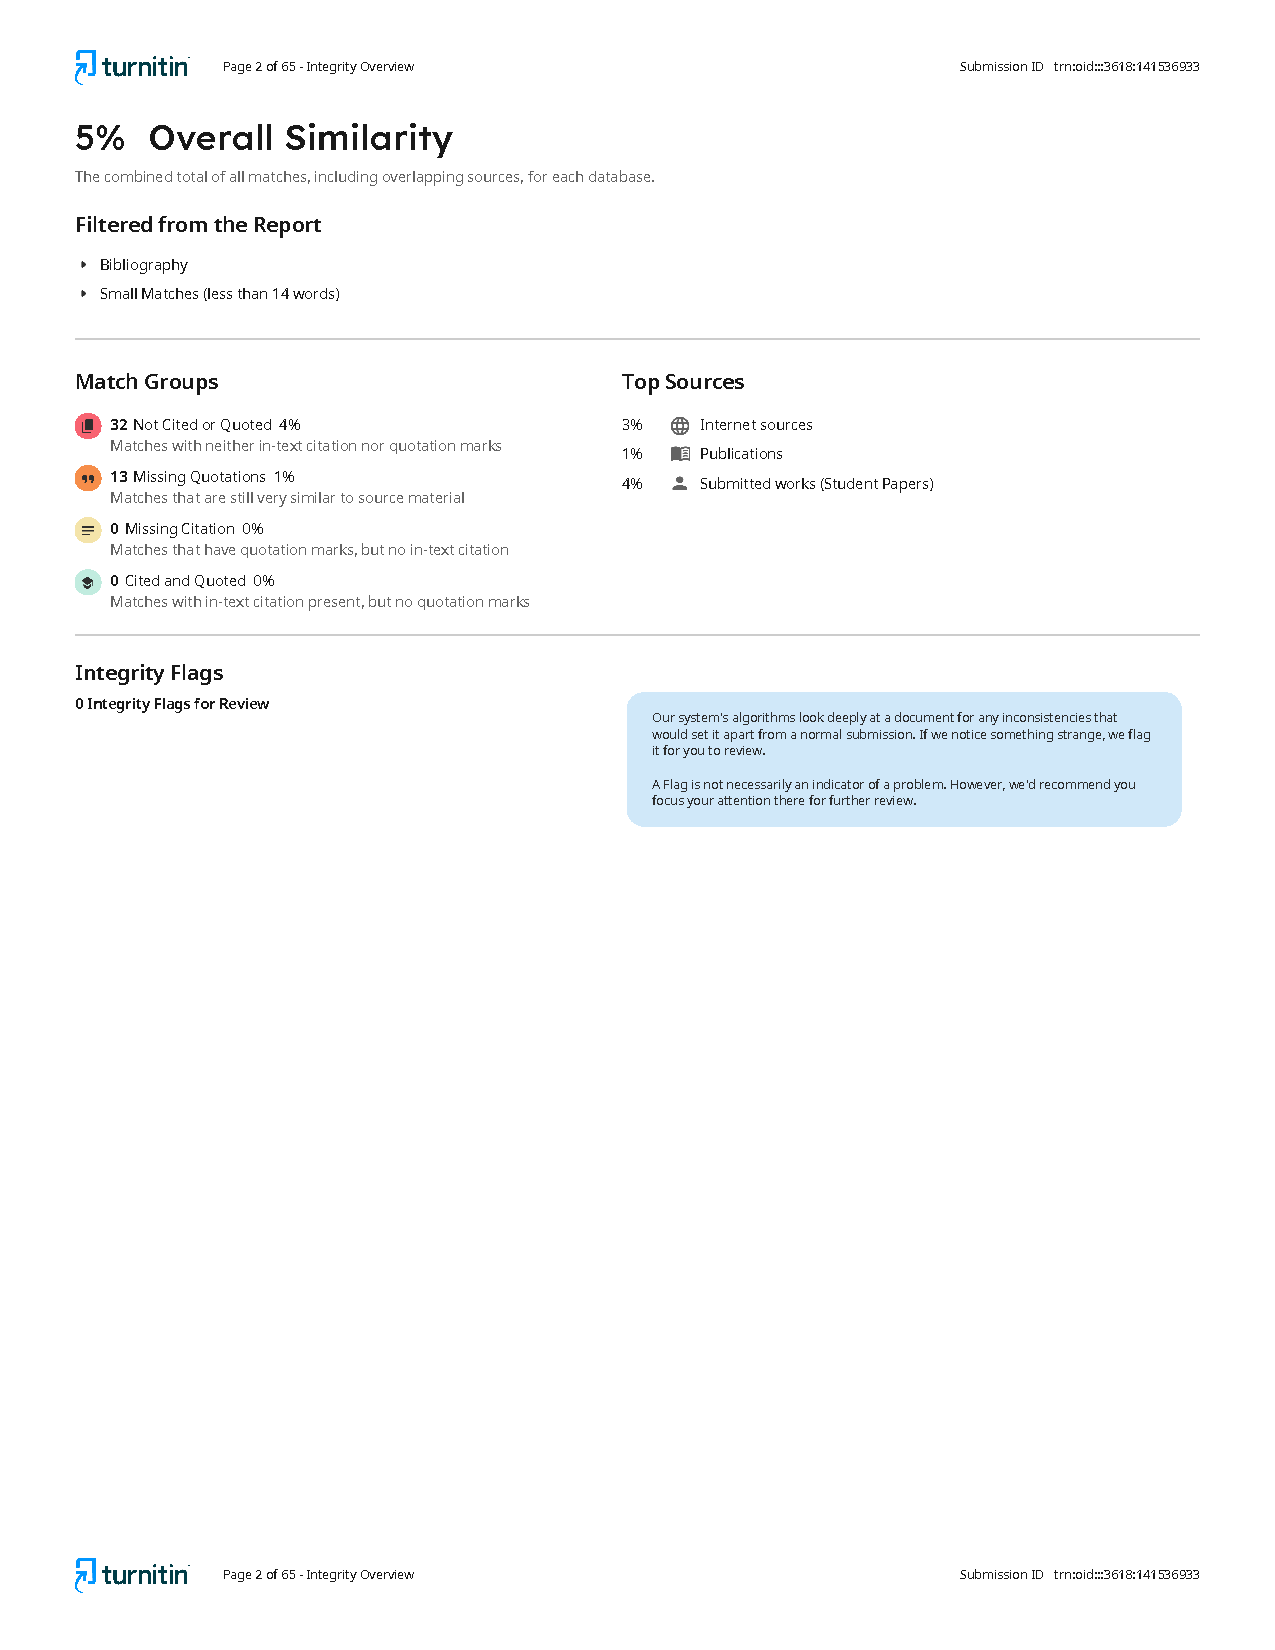
\includepdf[pages=-]{sep (2) (1)-2.pdf}

\end{document}

